\documentclass[oneside,numbers,english]{./ezthesis}
%% # Opciones disponibles para el documento #
%%
%% Las opciones con un (*) son las opciones predeterminadas.
%%
%% Modo de compilar:
%%   draft            - borrador con marcas de fecha y sin im'agenes
%%   draftmarks       - borrador con marcas de fecha y con im'agenes
%%   final (*)        - version final de la tesis
%%
%% Tama'no de papel:
%%   letterpaper (*)  - tama'no carta (Am'erica)
%%   a4paper          - tama'no A4    (Europa)
%%
%% Formato de impresi'on:
%%   oneside          - hojas impresas por un solo lado
%%   twoside (*)      - hijas impresas por ambos lados
%%
%% Tama'no de letra:
%%   10pt, 11pt, o 12pt (*)
%%
%% Espaciado entre renglones:
%%   singlespace      - espacio sencillo
%%   onehalfspace (*) - espacio de 1.5
%%   doublespace      - a doble espacio
%%
%% Formato de las referencias bibliogr'aficas:
%%   numbers          - numeradas, p.e. [1]
%%   authoryear (*)   - por autor y a'no, p.e. (Newton, 1997)
%%
%% Opciones adicionales:
%%   spanish         - tesis escrita en espa'nol
%%
%% Desactivar opciones especiales:
%%   nobibtoc   - no incluir la bibiolgraf'ia en el 'Indice general
%%   nofancyhdr - no incluir "fancyhdr" para producir los encabezados
%%   nocolors   - no incluir "xcolor" para producir ligas con colores
%%   nographicx - no incluir "graphicx" para insertar gr'aficos
%%   nonatbib   - no incluir "natbib" para administrar la bibliograf'ia

%% Paquetes adicionales requeridos se pueden agregar tambi'en aqu'i.
%% Por ejemplo:
%\usepackage{subfig}
%\usepackage{multirow}

\usepackage{graphicx,rotating,booktabs}
\usepackage{lscape}

%\usepackage[spanish]{babel}
\usepackage[spanish,USenglish]{babel} % espanol, ingles
%\usepackage[utf8]{inputenc} % acentos sin codigo
%\renewcommand{\chaptername}{chapter}
%\renewcommand{\tablename}{Table}
%\renewcommand{\figurename}{Figure}
\usepackage{multirow, array} %para mover el ancho de las tablas.
\renewcommand{\baselinestretch}{2}
%% # Datos del documento #
%% Nota que los acentos se deben escribir: \'a, \'e, \'i, etc.
%% La letra n con tilde es: \~n.
%0.15
\usepackage{vmargin}
\setpapersize{USletter}
\setmargins{3.2cm}       % margen izquierdo
{2.5cm}                        % margen superior
{15cm}                      % anchura del texto
{20cm}                    % altura del texto
{10pt}                           % altura de los encabezados
{1cm}                           % espacio entre el texto y los encabezados
{10pt}                             % altura del pie de página
{1cm}                           % espacio entre el texto y el pie de página


\usepackage{caption}
\usepackage{subfig}

\usepackage{amssymb, amsmath, amsbsy} % simbolitos
\usepackage{amsmath}
\usepackage{upgreek} % para poner letras griegas sin cursiva
\usepackage{cancel} % para tachar
\usepackage{mathdots} % para el comando \iddots
\usepackage{mathrsfs} % para formato de letra
\usepackage{stackrel} % para el comando \stackbin

%\usepackage{algpseudocode} %Para el apendice.
\usepackage{algorithm}
\usepackage{algorithmic}
\usepackage{listings}
%\usepackage{algpseudocode}
%\usepackage{pifont}

\usepackage[verbose]{placeins}
%\usepackage[ngerman]{babel}
\usepackage{blindtext}


%\usepackage[showframe,paper=a4paper,top=1in,bottom=1in,right=0.5in,left=1.5in]{geometry}% http://ctan.org/pkg/%geometry

%\author{Xochilt Ramirez Garcia}
%\title{ Sistema de Recomendaci\'on Sensible al Contexto y su Aplicaci\'on al Secuenciado de Objetos }
%\degree{Doctor en Ciencias en Computaci\'on}
%\supervisor{Nombre de mi Asesor}
%\institution{Instituto Tecnol\'ogico de Tijuana}
%\faculty{Divisi\'on de Estudios de Postgrado e Investigaci\'on }
%\department{Departamento de Sistemas Computacionales}

%% # M'argenes del documento #
%%
%% Quitar el comentario en la siguiente linea para austar los m'argenes del
%% documento. Leer la documentaci'on de "geometry" para m'as informaci'on.

%\geometry{top=40mm,bottom=33mm,inner=40mm,outer=25mm}

%% El siguiente comando agrega ligas activas en el documento para las
%% referencias cruzadas y citas bibliogr'aficas. Tiene que ser *la 'ultima*
%% instrucci'on antes de \begin{document}.

\hyperlinking
\begin{document}

\pagenumbering{Roman}
%\documentclass{article}
\usepackage{graphicx,rotating,booktabs}
\usepackage{vmargin}

\usepackage{geometry}
\geometry{letterpaper}

\setmargins{3cm}       % margen izquierdo
{2.5cm}                        % margen superior
{15cm}                      % anchura del texto
{22.5cm}                    % altura del texto
{10pt}                           % altura de los encabezados
{1cm}                           % espacio entre el texto y los encabezados
{10pt}                             % altura del pie de página
{2cm}                           % espacio entre el texto y el pie de página

\renewcommand{\baselinestretch}{2}

\begin{document}

\begin{center}
%\vspace*{\stretch{1.0}}
{\textsc{\LARGE \textbf{SEP} } \hfill  \textsc{\LARGE \textbf{TNM}}}\\[0.2cm]
	\textsc{\LARGE \textbf{INSTITUTO TECNOL\'OGICO DE TIJUANA}\\[0.5cm]
	\textsc{\Large Divisi\'on de Estudios de Posgrado }\\[0.1cm]
	\textsc{\Large e Investigaci\'on }}\\[0.5cm]
	% Upper part of the page
	%
\includegraphics[height=4cm]{img/logotec1.png}
	
\includegraphics[width=0.4\textwidth]{img/logotec1}\\[0.3cm] %0.15
	%\HRule \\[.2cm]
	{ \LARGE \bfseries Modelado de usuario para aplicaciones de evoluci\'on interactiva web utilizando navegadores y dispositivos m\'oviles}\\ [1.0cm]
\end{center}

 \begin{minipage}{1.0\textwidth}
 	\begin{flushright}
 	\textsc{Trabajo de tesis}\\[0.3cm]
 	\emph{Presentado por:} \\
 	\textsc{ M.C. Jos\'e Christian Romero Hern\'andez}\\
 	%\vspace{4 mm}}
	\emph{Para obtener el grado de:} \\
 	\textsc{Doctor en Ciencias en Computaci\'on} \\
 	%\vspace{4 mm}}
	\emph{Director:} \\
 	\textsc{Dr. Jose Mario Garc\'ia Vald\'ez} \\
 	\vspace{4 mm}
	\emph{Tijuana, B.C., septiembre 2017.}
 	\end{flushright}
\end{minipage}


\pagestyle{empty} % Removes page numbers


\end{document}

%% Los cap'itulos inician con \chapter{T'itulo}, estos aparecen numerados y
%% se incluyen en el 'indice general.
%%
%% Recuerda que aqu'i ya puedes escribir acentos como: 'a, 'e, 'i, etc.
%% La letra n con tilde es: 'n.

% 
%MG: En el resumen debes hablar de todo el trabajo revisa: 
%% http://www.slideshare.net/jjmerelo/cmo-escribir-y-publicar-trabajos-cientficos-17948694

% Da una breve introducción al tema (problema)
% Los métodos que pleanteamos aquí son {metodología}
% para [mejorar, evitar, comprobar] {problema}  
% Se probó de la manera {x} que los objetivos se alcanzaron  
% con los resultados siguientes {x} 

% Al integrar estas técnicas el desempeño mejoró en {x} respecto a {y}
% de manera estadísticamente significativa logrando para los datos de prueba 
% un error absoluto de XX.
% Es necesario comentar los resultados con el error?.. 

\prefacesection{Resumen}



\prefacesection{Abstract}











%% Los cap'itulos inician con \chapter{T'itulo}, estos aparecen numerados y
%% se incluyen en el 'indice general.
%%
%% Recuerda que aqu'i ya puedes escribir acentos como: 'a, 'e, 'i, etc.
%% La letra n con tilde es: 'n.

% 
%MG: En el resumen debes hablar de todo el trabajo revisa: 
%% http://www.slideshare.net/jjmerelo/cmo-escribir-y-publicar-trabajos-cientficos-17948694

% Da una breve introducción al tema (problema)
% Los métodos que pleanteamos aquí son {metodología}
% para [mejorar, evitar, comprobar] {problema}  
% Se probó de la manera {x} que los objetivos se alcanzaron  
% con los resultados siguientes {x} 

% Al integrar estas técnicas el desempeño mejoró en {x} respecto a {y}
% de manera estadísticamente significativa logrando para los datos de prueba 
% un error absoluto de XX.
% Es necesario comentar los resultados con el error?.. 

\prefacesection{Dedicatoria}



Dedico este trabajo a mi esposa Iliana Durón Landero por el apoyo incondicional
que brindaste durante todo el proceso. 
“Sabemos muy poco, y sin embargo es
sorprendente que sepamos tanto, y es todavía mas sorprendente que tan poco
conocimiento nos de tanto poder.” Bertrand Russell        
“Después de todo, cualquier tipo de conocimiento implica auto-conocimiento.” Bruce Lee 
“El conocimiento descansa no solo sobre la verdad sino también sobre el error.” Carl
Jung 
“El conocimiento depende del tiempo, mientras que el saber no. El
conocimiento es una fuente de acumulación, de conclusión, mientras que el saber
es un continuo movimiento.” Bruce Lee












%% Las secciones del "prefacio" inician con el comando \prefacesection{T'itulo}
%% Este tipo de secciones *no* van numeradas, pero s'i aparecen en el 'indice.
%%
%% Si quieres agregar una secci'on que no vaya n'umerada y que *tampoco*
%% aparesca en el 'indice, usa entonces el comando \chapter*{T'itulo}
%%
%% Recuerda que aqu'i ya puedes escribir acentos como: 'a, 'e, 'i, etc.
%% La letra n con tilde es: 'n.

\prefacesection{Agradecimientos} Agradezco al CONACYT por haberme brindado la
oportunidad y el apoyo a trav\'es de la beca 256554 durante el periodo de
Agosto-2011 a Agosto-2015 para concluir los estudios de Doctorado en Ciencias en
Computaci\'on.

A mi director de tesis, Dr. Jos\'e Mario Garc\'ia Valdez  que le tengo una
enorme gratitud por haberme ense\~nado herramientas tan valiosas para mi
formaci\'on como profesional as\'i como persona de tecnolog\'ia. Al Dr. Oscar
Castillo L\'opez y tambi\'en a la Dra. Elba Patricia Mel\'in por haberme
brindado la oportunidad de entrar al programa de doctorado en ciencias de la
computaci\'on del Instituto Tecnol\'ogico de Tijuana, a todos ustedes gracias
por su paciencia y recomendaciones para hacer posible este proyecto de tesis.


A mi familia, por su comprensi\'on y apoyo, en especial a mis padres, el Ing.
Julian Torres Ruiz, Lic. Susana Hern\'andez Velarde por haberme apoyado en el
cuidado de mi hija Victoria Alessandra Romero Dur\'on, ya que sin ustedes hubiera
sido imposible lograr esta meta.



\textit{}


%% # 'Indices y listas de contenido #
%% Quitar los comentarios en las lineas siguientes para obtener listas de
%% figuras y cuadros/tablas.
%\begin{singlespace}
\listoffigures
\listoftables
\tableofcontents
%\end{singlespace}
\clearpage
%\listoffigures
%\listoftables
%% # Cap'itulos #
%% Por cada cap'itulo hay que crear un nuevo archivo e incluirlo aqu'i.
%% Mirar el archivo "intro.tex" para un ejemplo y recomendaciones para
%% escribir.%\setcounter{page}{6}

\pagenumbering{arabic}
\chapter{Introduction} \label{introduction}


\par Interactive evolutionary computation (IEC) are methods where users replace the
fitness function in evolutionary methods \cite{eiben2015introduction}.
These methods usually apply to problems
where the fitness function is unknown or does not exist, and the result of the
optimization must be adjusted to particular needs, for example, the tastes or
desires of users. In that sense, the case study includes evolving objects
with individual characteristics, such as visual appeal as well as others where
human behavior is considered, such as optimization of teamwork
\cite{kosorukoff2002evolutionary} or creativity \cite{yu2011cooks}. In cases
where human interaction is  responsible for other aspects of the evolutionary
process, some authors classify it as evolutionary computation based on human
\cite{kosorukoff2001human} or human-based computation \cite{quinn2011human}.
Interactive evolutionary computing systems are an exciting field of research, as
they have demonstrated their ability to produce art and designs effectively
\cite{bentley1999introduction}\cite{kowaliw2012promoting}\cite{sims1991artificial}\cite{todd1994evolutionary}.

\par However, the need for human intervention leads to several challenges for
designers of such systems, for instance, evaluations are slow, costly and
scarce, there is also the fatigue of people caused by interactions
\cite{takagi1998interactive}. The boredom that arises when users evaluate large
numbers of phenotypes (individuals) as these are very similar or just not attractive. The
performance of these systems depends on the amount of user participation, to
reach more people, some of these systems are migrating to web-based applications
depending on the help of their visitors about search with either anonymous users
or with registered users. Some of these systems implement collaborative
techniques, where some users participate in the evaluation of individuals, this
method is called collaborative-IEC \cite{secretan2008picbreeder}\cite{seyama2016development}\cite{wagy2014collective}.

\par We believe that interactive evolutionary computing should follow a human-centered
design \cite{greenhouse2012human}, giving particular attention to volunteer
users, not only because of the explicit evaluations they perform and are
essential but because the interaction context affects the system as a whole.
Because users not only interact with the graphical interface, and with each
phenotype presented in the system, but also users interact with other users, as
well as the activities they perform for example storing a phenotype, see some
phenotype of a given collection of another known user, and so on.

\par Within these systems not all users are equal, because the human is a complex
entity \cite{mitchell2009complexity}. In this sense we could say that users 
evaluations do not have the same weight, since this entails
that those users with a greater participation have certain influence on others,
this would produce a
type of trend in the evolutions of the phenotype and is necessary to know who
has the highest level of participation in these systems. This problem can be
addressed in different ways, but we propose to use the fuzzy logic
\cite{Zadeh1973}\cite{TakagiSugeno1983}\cite{ohsaki1998input} in order to assign
a weight to users preferences according to certain criteria that are within the
interaction activities carried out by users such as activities, tasks,
evaluations of phenotypes and rankings.

\par Therefore this gives us the guideline to generate a fitness assignment
strategy which weighted users according to the interaction activities mentioned
above in these systems beyond just the number of evaluations performed and the
number of views of the users. This makes users with more participations have
greater value, and therefore other users see it as a leader user about their
participations.

\par This thesis argues that a graph based user model is a viable representation of
the interactions and relations of actions that exist between users
and the phenotypes of these systems. Such relations could be evaluate, share, delete,
store and visualize entities or phenotypes. Graph-based models are currently
used in social networks to
keep track of users' interactions with media objects, places, and other users
\cite{bondy1976graph}\cite{miller2013graph}\cite{holzschuher2013performance}. Users on
social networks (e.g., Facebook) are accustomed to expressing these
complex relationships in statements such as: "Christian and Iliana are eating on
Friday's." Another example of a graph representation for this kind
of systems is the W3C activity stream 2.0 specification used to
represent activities in social web applications.

\par The knowledge generated by the graph-based user model is used to know how users
behave in this type of system with respect to their participation, that is, we
can observe the information generated by each user. In this sense, this
information is used both as part of the fitness calculation of the phenotypes in
one of the inputs in a fuzzy system and is also used as usability elements
interface through the gamification technique\cite{huotari2012defining}\cite{deterding2011game}\cite{hickman2010total}\cite{mcgonigal2011reality} technique
implemented in this research is based on a rewards mechanism \cite{sutter2010browse}.
Generally rewards are granted according to the reputation that certain users
have in the system and are represented using a score system with points, levels and
leader-boards. Points or scores are rewards given to the accomplishments of
activities that need to be done by users. The levels are acquired according to
the points that are generated by users. Finally a leader-board is where a user position
is shown with respect to others. The above
techniques cause that users in certain way get engage in these kind of
systems, due to the competitiveness between them.

% You must state the problem here, something like.
% In order to increase user participation we propose a framwork etc.
% Im shure this is stated in other section so you just need to
% get it in here
\par The necessary intervention of users in interactive evolutionary computational
systems has inherent drawbacks arising from the very nature of the algorithms,
namely, the human fatigue caused by the interaction, and the boredom arising
when users evaluate a large number of artifacts. To tackle these issues, in this
research we propose a human-centered framework to model complex interactions on
these systems.

\par In this work a case study is presented, where a web application was
developed based on digital art where the objective of the application is to
evolve drawings. This study case has three different versions where each of them
is presented for use to different groups of users. The first version uses simple
interactive evolutionary computation techniques where users can only visualize
and evaluate phenotypes as well as access the application and have the
functionality to create collections of their creations, but there is no record
of their activities. Also the second version is based on the aspects of the
first one, but this generates information of the activities of the users such as
registration to the application, evaluate phenotypes, create collections and so
on, and the fuzzy logic paradigm is implemented. The third version is also
based on the aspects of the two previous ones but the difference lies in how we
generate the information of interactivity with the application, since this
generates the graph-based model and the rewards mechanism is implemented, which
refers to usability aspects such as gamification, all this is implemented to be
able to study the changes of participation that exists with respect to the other
versions mentioned above. This study case is exposed in detail to the readers in
order to understand the concepts and uses of the proposed framework.



\section{Outline}

\begin{itemize}
\item \textbf{Chapter 2}, describes an in-depth study of current and related
works, presenting a general overview of interactive evolutionary computation and
their evolution in the pass and recent years, also user model approaches and
finally the gamification paradigm. This study includes Interactive evolutionary
computations methods and techniques to understand how they work, as well as
common problems found in these systems. On the other hand this study also includes user
modeling methods in order to understand how to create and apply them for certain
applications. Finally we discussed a gamification paradigm to
understand how it work and subsequently apply this for the necessities of this
work.

\item \textbf{Chapter 3}, describes the fundamental
concepts that form the basis of the proposed human-centered framework.


\item \textbf{Chapter 4}, presents a human-centered framework for interactivity
Web-based applications, this proposed framework involves different paradigms in
order to increase user participation. This chapter also includes the overall
explanation of how the functionality the proposed framework works.

\item \textbf{Chapter 5}, the case study is presented along with the
explanation of the experimentation for this work. The experiments were realized
using several versions of the same application in order to see which of them
have most user participation.

\item \textbf{Chapter 6}, The results of the case study are presented. This
chapter includes all the data obtained from the experiments, these data are
presented to see which of the versions meets the best performance regarding the
increase of participation of users.

\item \textbf{Chapter 7}, finally the conclusions and future work of this
research are exposed.
\end{itemize}

At the end of this document includes appendices that describe
detailed technical aspects about installation EvoDrawings application on heroku
cloud service as well as the fuzzy if-the rules used in ED03 application.
 

\chapter{State of the art and background} \label{}
This chapter describes an in-depth review of current and related works,
presenting a general overview of Interactive evolutionary computation and their
evolution in the pass and recent years, also user model approaches, In the same
way some works were review that contain the fuzzy logic concept and finally
gamification paradigm is also review.


\section{Interactive Evolutionary Computation.}

This technology is branch of evolutionary computation. Based on subjective human
evaluation. Basically, this technique requires that the objective function is
replaced by a person (user) [12]. Takagi defines it as "A optimization
technology that uses human evaluation in the optimization system instead of a
human evaluation model. Simply stated, the interactive EC is an EC whose fitness
function is replaced by a human.  In figure \ref{fig:IEC} we show a general IEC
system.

\begin{figure*}
	\captionsetup{justification=centering,margin=2cm}
	\centering
	\setlength\fboxsep{0pt}
	\setlength\fboxrule{0.7pt}
	\fbox{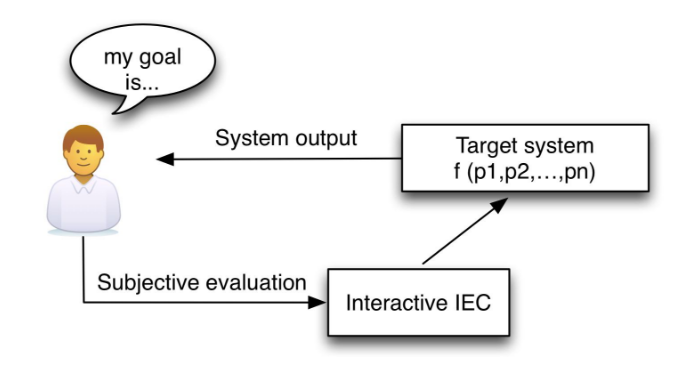
\includegraphics[width=10cm,height=10cm,keepaspectratio]{img/IECGeneral.png}}
	\caption{ General Interactive Evolutionary Computation system based on subjective evaluation.}
	\label{fig:IEC}
\end{figure*}



In this general IEC system we note that the user replaced the fitness function
at the moment he or she interacts with the system. Logically the user needs a
goal to know what is the evaluation he or she needs to perform. Finally the
users receive an output and the process and start over again.

These techniques have been used in several areas of application, in particular:
\begin{itemize}
	\item Music and sound.
	\item Digital Art.
	\item Design and editing documents
	\item Processing acoustic signals.
	\item Industrial design.
	\item Data mining and acquire knowledge.
	\item Face recognition.
	\item Robotics and control.
\end{itemize}

Below are some of the most outstanding works in the interactive evolutionary
computing area, which are the following:


Dawkins's research was the pioneer of a significant addition to the
1990s IEC algorithms research works\cite{dawkins1986blind}.

There is two key research approach about his field:

\begin{itemize}
	\item \textbf{Creative Approach:} The Artificial Life (AL) was the base of
	creative approach. AL uses complex algorithms for biological life models
	emulation. To perform this task, it is needed to include some of the different
	techniques starting from right image treatment. Good graphic creation as well
	as a great music and
	quality sounds, \cite{sims1991artificial}, \cite{sims1994evolving},
	\cite{dawkins1986blind}, \cite{disz1997ubiworld},
	\cite{unemi2000sbart}and \cite{unemi2003sbeat3}.
	\item \textbf{Humanized technology approach:} The concept of humanized
technology approach comes from the approach that is focused on the IEC
algorithms interface, this is the research of interaction between humans and
computer systems. The main goal of this was to reduce the user's fatigue and to
promote the inputs and outputs of algorithms to improve the efficiency of them.
IEC has made his own way in practical fields such as engineering,
education,etc.,
	\cite{parmee1993concrete}, \cite{ventrella1994explorations},
	\cite{takagi1996discrete}, \cite{poli1997genetic},
	\cite{parmee1998genetic} and \cite{takagi1998interactive}.
\end{itemize}




Computer graphics (CG) The Biomorph of Dawkins was the first IEC research, from
this research comes to many motivated works mostly about the Selfish Gene, come
of these works are:  \cite{ochoa1998genetic},
\cite{mccormack1993interactive}.

In Dawkins work, a conventional recursive algorithm was used as a baseline
maintaining the main target of trees with an L-system (Lindenmayer). This same
L-system was the base for another experiment to create 2-D CG forms insects from
a system called Blind Watchmaker who used L-system angles from L-system output
intuitively selected; the creation was called biomorphs. These creations reach
his target with the multiple selections of the users based on their preferences;
all these selections acted like a natural adaptation filter.

We can find plenty of applications and works for fractal generation and
\cite{sims1992interactive}, \cite{baluja1993simulating} and
\cite{baluja1994towards}, \cite{lund1995artistic}, or
\cite{angeline1996evolving},\cite{raynal1999manipulation}[Raynal 1999] and
\cite{lutton2003artie}, for rendering in tridimensional,
\cite{todd1992artificial},\cite{broughton1997use}, \cite{das1994genetic}[Das
1994] and \cite{tam2002genetic}, for generation of virtual creatures,
\cite{rowland2000evolutionary}, or aerodynamic surface design (wings),
\cite{nguyen1993evolvable}, \cite{nguyen1994evolvable} and \cite{}[NGuyen 1997].

We can discover more than one additional way to use this research in the
artistic field with several applications of IEC who are used for cartoon face
construction and animations matters, like Mutator \cite{todd1994evolutionary}
and \cite{todd1999mutation} or \cite{bentley1999introduction}.

The genetic programming (GP) applications offers a category called Interactive
Genetic Programming (IGP) with many examples of successful application in
tridimensional artwork for artistic animations or construction using
mathematical equations as CAVE \cite{das1994genetic},
\cite{papka1996ubiworld} and \cite{disz1997ubiworld},
\cite{sims1991artificial},
\cite{sims1992interactive} and \cite{min2004creative}. As
this work consequence, Panspermia or Primordial Dance was created that are
presented in figure \ref{fig:Panspermia} and figure \ref{fig:PrimordialD}.

\begin{figure*}
\captionsetup{justification=centering,margin=2cm}
\centering
\setlength\fboxsep{0pt}
\setlength\fboxrule{0.7pt}
\fbox{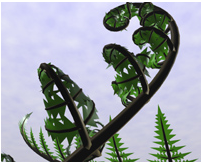
\includegraphics[width=10cm,height=10cm,keepaspectratio]{img/Panspermia.png}}
\caption{Panspermia.}
\label{fig:Panspermia}
\end{figure*}

\begin{figure*}
\captionsetup{justification=centering,margin=2cm}
\centering
\setlength\fboxsep{0pt}
\setlength\fboxrule{0.7pt}
\fbox{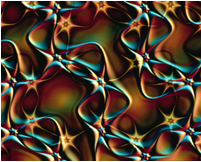
\includegraphics[width=10cm,height=10cm,keepaspectratio]{img/PrimordialDance.png}}
\caption{Primordial Dance.}
\label{fig:PrimordialD}
\end{figure*}


The artistic field is only the first step of a great IEC implementation; it is
important to mention another relevant projects called Galapagos,
\cite{sims1997interactivity}, and SBART, \cite{unemi2000sbart}. The IEC
application Galapagos Project is the exhibit in Tokio Multimedia Museum, (NTT
Intercommunication Center) and this project originates engaging images to all
visitors based on L-systems as we can see in figure \ref{fig:Galapagos1} and
figure \ref{fig:Galapagos2}.

\begin{figure*}
\captionsetup{justification=centering,margin=2cm}
\centering
\setlength\fboxsep{0pt}
\setlength\fboxrule{0.7pt}
\fbox{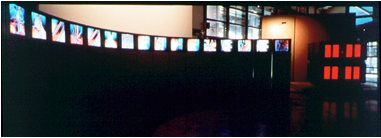
\includegraphics[width=10cm,height=10cm,keepaspectratio]{img/Galapagos1.png}}
\caption{Galapagos: Tokio Multimedia Museum.}
\label{fig:Galapagos1}
\end{figure*}

\begin{figure*}
\captionsetup{justification=centering,margin=2cm}
\centering
\setlength\fboxsep{0pt}
\setlength\fboxrule{0.7pt}
\fbox{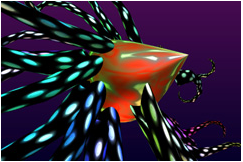
\includegraphics[width=10cm,height=10cm,keepaspectratio]{img/Galapagos2.png}}
\caption{Galapagos' output sample.}
\label{fig:Galapagos2}
\end{figure*}

There are created after one selection, to get a good solution through multiple
repetitions. This action is performed with Genetic Programming (GP), after the
calculation of each pixel value using trees of equations combining logarithm,
maximum, and minimum, sine, root, cosine, exponential arithmetic operators.
AnimationLab is found as an outstanding work who offer figures that can run or
walk working with the user to receive more opportunities to be picked. A
particular characteristic of all of the figures is that the figures extremities
Mentioning open source works, we can find SBART as an IGP
\cite{unemi2000sbart} tool to create graphics. SBART allow to users
to evaluate 20 two-dimensional images, subsequently twenty new image has
direction and angles as we can see in figure \ref{fig:AnimationLab}.

\begin{figure*}
\captionsetup{justification=centering,margin=2cm}
\centering
\setlength\fboxsep{0pt}
\setlength\fboxrule{0.7pt}
\fbox{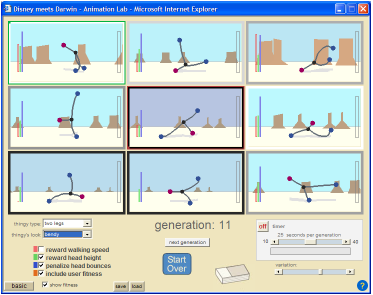
\includegraphics[width=10cm,height=10cm,keepaspectratio]{img/AnimationLab.png}}
\caption{Animation Lab.}
\label{fig:AnimationLab}
\end{figure*}

There are many examples for this field application as
\cite{mckenna1990dynamic},
\cite{ventrella1994explorations}, or
\cite{ventrella1995disney}, \cite{lim1999pro} and
\cite{lim2000solve}.  One of the Interactive Evolutionary Programming
(IEP)  artistic application was created by \cite{angeline1996evolving}, as a fractal generation where the system allows the evolution of
animations for the ones who were selected from the user, the application
initially show only 10 animations to rate.


It is important to know how IEC was implemented in music generation, with
several applications in this field. We will start mentioning the pioneer
application GENJAM, \cite{biles1994genjam},
\cite{biles1996neural} or \cite{biles1999life} and
\cite{biles2002genjam}. Some other attractive works are Sonomorph,
\cite{nelson1993sonomorphs} and \cite{nelson1995further}, or SBEAT, \cite{unemi2003sbeat3},
\cite{horowitz1994generating}, \cite{onisawa2000composition}, \cite{tokui2000music} and
\cite{fels2002interactive}. It is possible to hear a part of the
music songs of these previously mentioned works broadcasted in the radio station
WDYN. (100.1, New York, USA, WEBPage:http://www.wdyn.net/).

The IEC algorithms are the base for the functionality of the music generation
systems, a visual representation of this is given in the below figure \ref{fig:GENJAM}:

\begin{figure*}
\captionsetup{justification=centering,margin=2cm}
\centering
\setlength\fboxsep{0pt}
\setlength\fboxrule{0.7pt}
\fbox{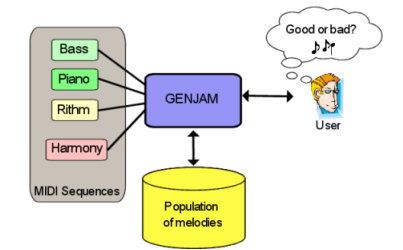
\includegraphics[width=10cm,height=10cm,keepaspectratio]{img/GENJAM.png}}
\caption{GENJAM squeme.}
\label{fig:GENJAM}
\end{figure*}

In 1998, a new input method for human operators of an interactive genetic algo-
rithm to reduce the psychological weight is proposed. This method uses a
discrete fitness values to reduce the psychological stress involved in the input
procedure. They perform simulations to investigate the influence of the
resulting quantization noise from the use of discrete values of fitness in
convergence. Showing that the quantization noise does not significantly worsen
in the convergence. In this method they evaluated using two subjective tests
involving the task of drawing faces.

The subjective test results shows that this method significantly reduce the
level of psychological stress of human interactive genetic algorithms operators
\cite{ohsaki1998input}. Another approach, proposed to used novel method
evaluation. Where the user only evaluates a satisfactory or unsatisfactory
individual. These approach consider the level of sensibility of the different
users to their perception of the beautiful and the ugly, and fitness is
automatically calculated based on user evaluations and time. They also propose
effective strategies for comparing different individuals of the same generation
in uncertain fitness conditions of an individual. Where they obtains the
probability of an individual dominance by use of the probability of the interval
domain, and translate to a fuzzy number in a range based on α-cut set
\cite{gong2009impact}. They determine the dominant individual in tournament
selection with size being two on base given by the probability of a particular
domain. This approach was applied to an interactive evolutionary system for
fashion design. In figure 1 we can see different user interfaces they used.
Based on this approach, another work was de-rived. Where the approach adopt a
fuzzy number described with a Gaussian membership function to express an
individual's fitness. In order to compare the different individuals, they
generated a fitness interval based on a cut set, and obtain the probability of
interactive genetic algorithms with individual's fuzzy fitness. The
contributions in this approach can improve the performance of existing income
generating activities in alleviating user fatigue and finding optimal solutions
to an optimization problem, so it is beneficial for solving complicated problems
with implicit or fuzzy indices \cite{gong2011interactive} we can see the user
interface in figure \ref{fig:fashion}.

\begin{figure*}
\captionsetup{justification=centering,margin=2cm}
\centering
\setlength\fboxsep{0pt}
\setlength\fboxrule{0.7pt}
\fbox{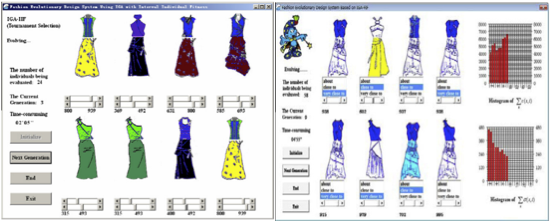
\includegraphics[width=10cm,height=10cm,keepaspectratio]{img/fashion.png}}
\caption{Different user interfaces interactive evolutionary system for fashion design.}
\label{fig:fashion}
\end{figure*}

\subsection{Web-Based IEC aplications .}


\subsubsection{Picbreeder.}
Picbreeder is a Web-based application that allows users to evolve images in a
col-laborative way maintaining a large catalog of user-created content allowing
users collaboration by searching through extensive design spaces
\cite{secretan2008picbreeder}. Picbreeder provides to users of all
experience levels to enjoy all the creative contributions produced by other
users. In this way users experience a new form of recreation called creative
social recreation through collaborative exploration. In this sense these systems
helps their users to find interesting images through tagging, browsing and
searching as figure  \ref{fig:Picbreeder} show.

\begin{figure*}
\captionsetup{justification=centering,margin=2cm}
\centering
\setlength\fboxsep{0pt}
\setlength\fboxrule{0.7pt}
\fbox{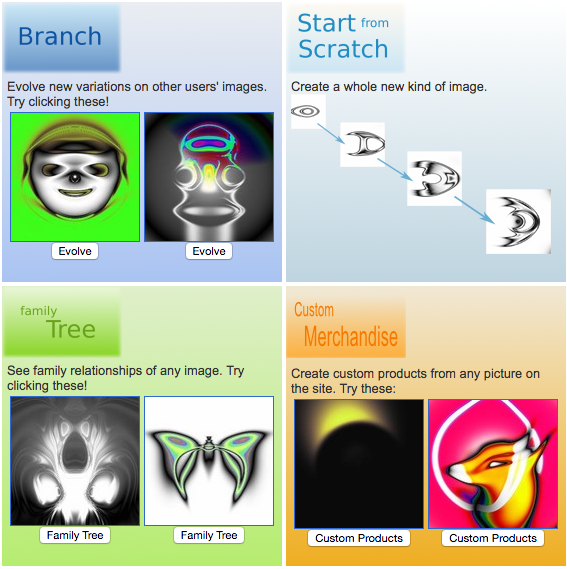
\includegraphics[width=10cm,height=10cm,keepaspectratio]{img/Picbreeder.png}}
\caption{Picbreeder User Selection.}
\label{fig:Picbreeder}
\end{figure*}

\subsubsection{EndlessForms.}
EndlessForms is a Web application that Explore object designs by choosing those
the users like. These selected objects become the parents of the next generation
of objects \cite{clune2011evolving}. EndLessForms proposes a new way to evolve
3D objects inspired by biological morphologies using generative encoding. One of
the experiments proposed in this paper was to use interactive evolutionary
systems to determine the potential for generating complex and interesting 3D
objects. They chose the interactive evolution, because that allows openended
exploration of the design space of objects that can produce by their method.
Additionally, the interactive evolution avoids the greedy nature of evolution by
objectives, which potentially allows to access more interesting objects
\cite{clune2011evolving}. In figure \ref{fig:EndlessForms} we can see some of
this objects.

\begin{figure*}
\captionsetup{justification=centering,margin=2cm}
\centering
\setlength\fboxsep{0pt}
\setlength\fboxrule{0.7pt}
\fbox{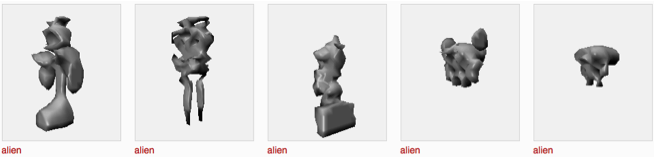
\includegraphics[width=10cm,height=10cm,keepaspectratio]{img/EndlessForms.png}}
\caption{Alien objects from EndLessForms.}
\label{fig:EndlessForms}
\end{figure*}

\subsubsection{EvoSpace-Interactive} EvoSpace-Interactive is an open source
framework focused on Web environments for collaborative interactive evolutionary
applications. This framework defines three main components for each application,
which are:
\begin{itemize}
	\item Individual.
	\item Processing Script.
	\item Worker Script.
\end{itemize}

The individual is represented internally as a data dictionary stored in Redis
[16] database management system; the individual contains main attributes as id,
chro-mosome, mom, dad, and views. This attributes represents the key information
of the individual as the individual offspring, the number of times that the
individual has been selected, etcetera, as we can see in figure \ref{fig:individualRep} [3].

\begin{figure*}
	\captionsetup{justification=centering,margin=2cm}
	\centering
	\setlength\fboxsep{0pt}
	\setlength\fboxrule{0.7pt}
	\fbox{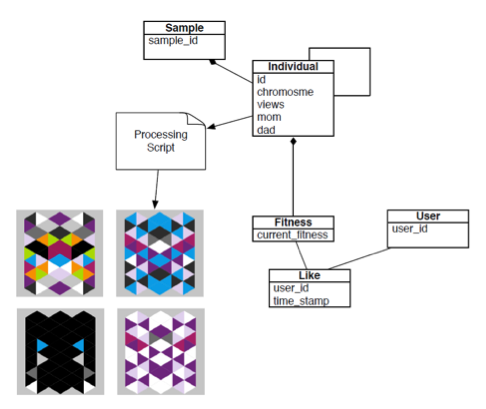
\includegraphics[width=10cm,height=10cm,keepaspectratio]{img/individualRep.png}}
	\caption{Individual Representation.}
	\label{fig:individualRep}
\end{figure*}

As we can observe on figure \ref{fig:ESFramework}, this work uses database
management systems to implement collaborative interactive evolutionary
applications. One of the reasons that this framework is using Redis[15] is
because it provides a hash- based imple-mentation of sets and queues, which are
natural data structures for the EvoSpace model. On the other hand this framework
uses a relational database to save basic information about the user extracted
from the social platform (Facebook) through open graph API and OAuth2
authentication.
\begin{figure*}
	\captionsetup{justification=centering,margin=2cm}
	\centering
	\setlength\fboxsep{0pt}
	\setlength\fboxrule{0.7pt}
	\fbox{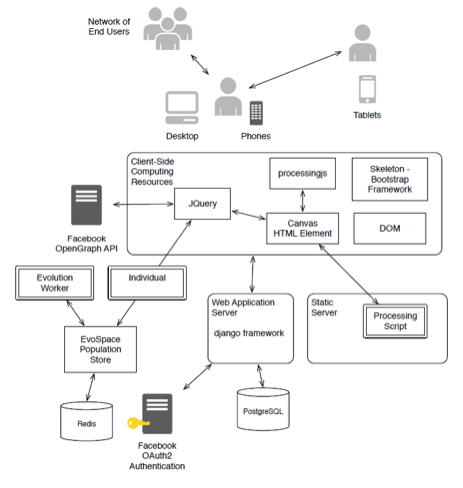
\includegraphics[width=10cm,height=10cm,keepaspectratio]{img/ESFramework.png}}
	\caption{EvoSpace-Interactive Framework.}
	\label{fig:ESFramework}
\end{figure*}

\section{User Modeling}

%%\subsection{Traditional Production Systems}

User modeling can be represented as the technique of building a model of the
user to personalize a system. The user model is commonly created as the user is
working with the system. An example is an educational application that teaches
students an individual skill: given the rules and knowledge in the user model,
the difficulty level of the exercises in the form is altered as the user
progresses.   Formally definition of user modeling according to McTear
\cite{mctear1993user} : " user modeling is the process of gathering information
about the users of a computer system and of using the information to provide
services or information adapted to the specific requirements of individual users
(or groups of users)". The purpose of the user model is to have a module
containing the operations that are needed to personalize the system, and the
user profile, which includes the personal data of the user \cite{}( Mohamad et
al., 2013).    System personalization over user modeling is related to the
research field of adaptive systems; this subject is beyond the scope of this
research work. Focus on the human user, user modeling is a very
cross-disciplinary research topic, comprehending the domains of artificial
intelligence, computer science, and social science. Ideas have been co‐opted
from an extensive range of subdomains, such as human–computer interaction,
e‐learning, information science, social computing, machine learning, data
mining, cognitive science, and so on \cite{kay2012coming}
\cite{kobsa2001generic}. There is interest in user modeling from both a
scientific and commercial perspective \cite{razmerita2009user}.

\subsection{Application Domains for user modeling}

Amount Research and implementation exist in this domain in which personalization
and user modeling plays an important role. This section presents several works
of these domains. To understand this topic, the different objects are divided
into three general categories:
\begin{itemize}
	\item {supporting a user during a task. }
	\item {giving a user a specific personalized experience. }
	\item {training and educating a user.}
\end{itemize}
The categories especially differ in the kind of user data that is used. For each
domain, the general purpose of the domain and the more accurate purpose of the
user model are discussed.

\subsection{User models for providing task support}

Task support systems are f systems that help a user during a task by either
supporting the user perform the task or by completely taking over this task
\cite{brun2010compass}(Nurmi et al., 2007). For instance,  an application that
automatically categorizes the incoming emails of the user. The goal of the user
model in these requests is to promote the efficiency of interactions with the
user, to simplify these interactions and to make complex systems more usable
\cite{razmerita2009user}\cite{fischer2001user}.
To perform this personalization, data is
collected through observations of the user. This information is related to the
user’s goals and needs, but especially to the task that the user currently is
accomplished, like the user’s task knowledge and background. Much research has
been done in this domain, but because many separate research projects are
focusing on an exact task or subject \cite{}(Sannes, 2011), it is hard to make
generalizations or to establish one delimited investigation topic. Commonly
discussed research subjects are Decision Support Systems,  Adaptive Hypermedia,
and Adaptive Ubiquitous Systems, each having his or her own specific domain and
way of personalization.

\subsection{Decision support systems}

Decision support systems are systems that support a user with making a decision
in a complex, professional environment \cite{} (Nurmi et al., 2007). For example,  a
system used at a pharmacy for automatically checking valid combinations of
medicine. The method can be used to help the pharmacist in prescribing the right
combinations and to give information for making a decision when a problem
occurs.  The purpose of the user model in decision support systems is to present
the user with the right and appropriate information, giving different feedback
or applying various decision steps according to the characteristics of the
user.The data that is used is often associated with the user’s task and
background knowledge.    The adaptation takes place by adapting the amount and
the content of the feedback provided by the system.


Decision support systems are traditionally ruled ‐ or logic-based systems, in
which all the relevant information is represented in a knowledge base. This
means that the content of the user model itself is also highly dependent on the
way the rules and knowledge are represented.


\subsection{Adaptive Hypermedia}

Adaptive hypermedia system is a system that grant users to browse freely
information network,  structured by nodes and links, to retrieve items of
information \cite{deepa2012adaptive}. For instance an internet website
application. The goal of the user model is to make the interface and structure
of the system dynamic. This enables the application to adapt to the user and to
make it easier for the user to search for and retrieve relevant information.
The data used in the user model is related to the user’s abilities, knowledge,
and goals in the application. The adaptation happens by adjusting the structure
and the presentation style to the expected needs of the user. For example, by
enhancing web search: promoting pages that might better correspond to the user’s
characteristics, on the other hand by giving navigation support, through
highlighting certain components of a page \cite{razmerita2012user}.

\subsection{User models for providing a personal experience.}

User models for providing the user with a personal experience have the goal to
improve the user experience while using the system.  This kind of user modeling
is especially focused on more commercial fields, such as e-commerce, marketing,
and computer games, and became popular with the rise of the Internet.  The
information that is used by the user in this main domain is mostly focused on
the information that defines the user, such as the user’s preferences and
interests. Since this data is regularly delicate, privacy is a  big issue
\cite{toch2012personalization}. While in other domains the privacy of the user
data is also important, in this area it is even a greater topic of discussion
because the incentive of the application developers is frequently contradictory
to the incentive of the actual user, considering gaining and sharing the user´s
personal information. For instance, user profiles are often shared among diverse
components of the same application, or even with different applications
\cite{brun2010compass} \cite{karam2012modeling}, which presents additional
weaknesses and possible undesirable information sharing.  Ensuring personal data
is not open to all people, in addition to defining strict privacy policies, is
thus essential in these user models. Some investigation in this domain are.

\subsection{Recommender Systems and User Adaptive Computer Games.}

Recommender systems are concerned with presenting the user with relevant
information and suggestions. They are commonly used on the Internet, for example
on websites such as Facebook, to provide the user with personalized news,
targeted advertisements and possibly new friends \cite{brun2010compass}. The
purpose of the user model is to give the system with information that is assumed
to be important for the user. The information that is stored for this goal is
associated with the preferences of the user to certain objects, like products,
music or people. To benefit a classification of these objects, the interaction
history of the user is stored, or the user is explicitly asked to rate certain
objects. The content of the system is eventually adjusted by showing the
recently inferred objects. In these senses, objects can be inferred by looking
at the attributes of the objects in the user profile, or by looking at the
objects in other user profiles that are related to the user \cite{kobsa2001generic}
\cite{kay2012coming}.  As a result of the predominantly commercial target of these
systems, the adaptations often take place in a very invasive way, to make sure
the user notices the change. Most recommender systems are based on the Internet,
which means that some typical technical difficulties  are associated with these
kinds of user models. First, the user profile is often only stored while the
user’s visit,  which means that fast and efficient adaption is important.
Recommender systems usually become more precise  when the user spends more time
with the system. Second, the system’s architecture is usually client-server,
where the client side gathers user information and sends it to the server, where
the  actual process takes place.

\subsection{User Adaptive Computer Games.}

User Adaptive computer games are games that focus on increasing the perceived
value by providing a strongly individualized experience (Brisson, 2012).  For
example is a first‐person shooter that adapts the performance of the enemy
according to the shooting accuracy of the player.

The fundamental idea of the user model is to identify or classify the user, so
the appropriate adjustment is made in the computer game. The information that is
used addresses the preferences and progress of the user, such as the user´s
current  difficulty level or even the employed strategy. This data is usually
obtained through the interactions of  the user with the game, and therefor first
should be translated and formalized  before it can be  used to interpret
conclusions on a higher level. The adaptation that takes place in the game
concerns changing the content and role of the  game, such as the game
difficulty, the behavior of non‐player characters  or even the background  music
\cite{bakkes2012personalised}.

Because of the emphasis on the user, user adaptive computer games have
relatively a lot of processing power available  for personalization. In this
sense the user adaptive computer games domain is a very interesting research
domain.



\subsection{Adaptive Educational Games.}

Adaptive Educational Games (AEGs) are complicated educational games that combine
ideas from several investigations areas, to increase the student’s learning
experience \cite{peeters2012situated}. These are especially based on  serious
games: computer games with an educational approach, where things are taught to
students by using a  playful idea \cite{korteling2011transfer} \cite{johnson2005serious}.
For instance an AEG is a training application  for fire fighters, letting
the fire fighters train their skills and knowledge in a safe on a virtual
environment.

The objective of the user model in an AEGs is to optimize the learning process
and outcome.   The user information is considered with the advance and knowledge
of the student, but also with the  student’s mental and cognitive
characteristics. The gained data can be used to adjust the content,
presentation, and system behavior to the  student’s need, for example, by
adjusting the content, tone, or amount of presented feedback. Adaptive computer
games have a lot of processing power available for personalization,  making a
complex and interesting domain for user modeling.

\subsection{Methods for user modeling.}

In the user modeling topic, researchers have proposed more general design
methods and frameworks to guide the developers in the process of user modeling.
These general methods are useful in research projects, where the knowledge can
be reused to adjust the user model to the system’s characteristics. Also in
commercial applications,  these general methods have proven to be useful
\cite{brun2010compass} , because they make it easier and more feasible to implement
personalization into a system. In early work, the process of user modeling was
mostly based on the intuition and experience of the developer or researcher. In
recent work, the techniques of user modeling were essentially based on the
intuition and expertise of the developer or researcher. As the user modeling
research field evolved, there has been put much effort in creating a general way
for designing and constructing a user model, by basing decisions on more
empirical grounds and by defining methods applicable to the whole field
\cite{kobsa2001generic} \cite{durrani1997cognitive}.

Frameworks,  methodologies, and architectures have been developed, defining the
strict process, restrictions and choices on how to design and build a user
model.  In the early days of user modeling, the focus was put on developing one
method applicable to the user modeling field as a whole. However, user modeling
is a very cross‐disciplinary research subject. Therefore, throughout the
decades, the user modeling area of research has been influenced by the important
research topics and trends of their time. For example, when information
technologies became a major subject in the early nineties, user modeling methods
were also mostly focused on the application of stereotypes, knowledge bases, and
logic to define a user model. With the rise of the Internet, the objectives of
the user modeling field change to Web-oriented applications and all the specific
problems that arise with this. Thus this connection,  also the general user
modeling methods that were developed, were focused on the popular research
domains of their time \cite{kay2012coming}. The main approaches to user modeling
did not change, but the specific filling‐in of the user model, such as which
technology to apply, did change. In this sense development of user modeling as a
whole, most researchers eventually agreed that one method to solve all problems
is not possible \cite{mctear1993user} \cite{kobsa2001generic}. Instead, a broad
range of  generic user modeling methods has been developed
\cite{fischer2001user}; each of which supports only a few of the very different
manifestations of personalization.



\section{Gamification.}

A definition given by Huotari  \cite{huotari2012defining} is  “Gamification is
the process by which concepts are brought to the real world task associated with
real people”. Also gamification handle game design elements which are commonly
known as non-game context in the presud to  enhance user engagement,
organizational productivity, flow, learning, evaluations, among others.

Games and game technologies increase exponentially the traditional boundaries of
their medium, as evidenced by the growth of serious and pervasive games as an
industry and research field. The most recent phenomenon in this path is
‘gamification’, paradigm for the use of video game elements (rather than full-
fledged games) to improve user experience and user engagement in non-game
services and applications \cite{deterding2011gamification}.

\subsection{Techniques.}


Techniques in this context seek to persuade users to use their natural desire to
compete, learn and socialize in given non-game context application
\cite{deterding2011game}\cite{hamari2014does}.  Some works in the beginning used
rewards for users as players to perform desired tasks in a certain application
or involving users to compete with each other . For instance some sort of
rewards include points \cite{sutter2010browse}, achievement badges or levels
\cite{hamari2011framework}, the filling of a progress bar \cite{o2010get}, or
providing the user with virtual currency. By Making the rewards for  tasks
achievements visible to other players or providing leader boards are ways of
encouraging players to compete \cite{hickman2010total}. Because the  problematic
consequences of competition, which can result in negative conduct, low
cooperation and collaboration, or disadvantaging certain player demographics
such as women \cite{kumar2013gamification}, best-practice gamification designs
try to refrain from using this element.

Another techniques to gamification is to make existing tasks feel more like
games \cite{deterding2010just}. Some techniques used in this approach include
adding meaningful choice, onboarding with a tutorial, increasing challenge, and
adding narrative \cite{mcgonigal2011reality}.

%%%% La letra n con tilde es: 'n.

\chapter{Background}

This chapter present the fundamental concepts related this work. The
formal definitions referring to fuzzy systems, contextual factors and
recommender system techniques used in the proposed method.
%--------------------------------------------------------------
%Agregue la seccion de logica difusa del articulo que me mando.
\section{Production systems and fuzzy models}

\subsection{Traditional Production Systems}

Production Systems represent knowledge in form of rules, which specify
actions that will be executed when certain conditions are met. Experts
in certain domain identify a set of rules based on their experience to
resolve different kinds of problems. Also known as rule based systems,
many implementations consist mainly of these three
components \cite{brachman1992knowledge} \cite{konar2006computational}:
\begin{enumerate}   
\item \textbf{Production Rules (PR)}. A set of
production rules (also known as IF-THEN rules) having a two part
structure; the antecedent, conformed by a set of conditions and a
consequent set of actions. 
\item \textbf{Working Memory (WM)}.
Represents the current knowledge or facts that are known to be true so
far. These facts are tested by the antecedent conditions of the rules
and the consequent part can change them. 
\item \textbf{Inference Engine (IE)}. 
This interpreter matches the conditions in the
production rules with the data/instantiations found in the WM,
deriving new consequences.
\end{enumerate}
The basic operation of these systems is described as a cycle of 
three steps \cite{brachman1992knowledge}:
\begin{enumerate}
\item \textbf{Recognize}: Find which rules are satisfied by 
the current WM. The antecedent part of the productions consists 
of a set of clauses connected by AND operators, when all these 
clauses have matching data on the WM the production has a chance 
of firing.
\item \textbf{Conflict Resolution}: Only one production can be 
fired at a time, so when two or more rules can be fired concurrently 
a conflict occurs. Among the production rules found in the first 
step, choose which rules should fire.
\item \textbf{Actions}: Change the working memory by performing 
the actions specified in the consequent part of all the rules 
selected in the second step. Changes occur by adding or 
deleting elements of the WM.
\end{enumerate}

This cycle continues until no further production rules can be fired.
This control strategy is data driven because whenever the antecedent
part is satisfied the rule is recognized, this strategy is also named
chain-forward. Other strategy is chain-backward in this case the work
is done from the conclusion to the facts, to chain-backward, goals in
working memory are match against consequents of the production
rules.\\  A drawback that has been recognized in these traditional
productions systems, is that some times rules are not fired in the
Recognize step because no appropriate match exists in the WM. Partial
matching of rules is not possible and this can be a limitation in some
systems because premature termination of the cycle is not desired. An
approach to handle partial matching is using fuzzy logic
\cite{konar2006computational}. In the next section a review of the
extension of production systems with fuzzy logic is preasented.\\

\subsection{Fuzzy Production Rules}

Fuzzy production rules use fuzzy logic sets to characterize the
variables and terms used in the propositions of the rules. Fuzzy
production rules or fuzzy \textit{IF-THEN} rules are expressions of
the form \textit{IF} antecedent \textit{THEN} consequent, where the
antecedent is a proposition of the form \textit{"x is A"} where
\textit{x} is a linguistic variable and \textit{A} is a linguistic
term. The truth value of this proposition is based on the matching
degree between \textit{x} and \textit{A}. Propositions are connected
by \textit{AND}, \textit{OR} and \textit{NOT} operators. Some
implementations of fuzzy rule-based systems also include other kinds
of data types in their propositions, for example the FLOPS system
includes fuzzy numbers, hedges, and non fuzzy data types (integers,
strings and float) \cite{siler2005fuzzy}. Depending on the form of the
consequent, two main types of fuzzy production systems are
distinguished \cite{babuvska1996fuzzy}:
\begin{itemize}  
\item \textbf{Linguistic fuzzy model}: where both the antecedent 
and consequent are fuzzy propositions.
\item \textbf{Takagi-Sugeno fuzzy model}: the antecedent is a fuzzy 
proposition; the consequent is a crisp function.
\end{itemize}  
As before, other non-fuzzy consequents can also be implemented, like
the execution of commands or the addition of new data.\\
\textbf{Linguistic Variables (LV)} are variables that can be assigned
linguistic terms as values, i.e. if we define a linguistic variable
\textit{SPEED} we can assign it the linguistic terms \textit{SLOW},
\textit{MEDIUM} or \textit{FAST}. The meaning of these linguistic
terms is defined by their membership functions (MF). \textit{LV} can
be defined as a \textit{5-tuple} \textit{LV=}$<v,T,X,g,m>$ where
\textit{v} is the name of the variable, \textit{T} is the set of
linguistic terms of \textit{v, X} is the domain (universe) of
\textit{v,g} is a syntactic rule to generate linguistic terms,
\textit{m} is a semantic rule that assigns to each term \textit{t} its
meaning \textit{m(t)}, which is a fuzzy set defined in \textit{X}.

\subsection{Fuzzy Inference Systems}

\textit{Fuzzy Inference Systems} (FISs) also called \textit{Fuzzy
Models} are fuzzy production systems used for modeling input-output
relationships. From this input-output view, Babuŝka
\cite{babuvska1996fuzzy} describes these systems as \textit{"flexible
mathematical functions which can approximate other functions or just
data (measurements) with a desired accuracy"}. Fuzzy Productions Rules
define the relationship between input and output variables. Input
variables are defined in the antecedent part of the rule and the
consequent part defines the output variables. These FIS are used
mainly in control systems, and are basically composed of five
modules\cite{babuvska1996fuzzy}:
\begin{enumerate}  
\item \textbf{Rule Base.} The set of fuzzy production rules.
\item \textbf{Database.} Where the membership functions are defined.
\item \textbf{Fuzzy Inference Engine.} This module executes the 
fuzzy inference operations.
\item \textbf{Fuzzifier.} This interface transforms the inputs 
of the systems (numerical data) into linguistic values.
\item \textbf{Defuzzifier.} This interface transforms the fuzzy 
results into numerical data.
\end{enumerate}
Usually the Rule Base and Data Base modules are collectively 
called the Knowledge Base module. The steps involved in fuzzy 
inference in a FIS are \cite{dubois1980fuzzy}:
\begin{enumerate} 
\item Compare the input variables with the membership functions 
in the antecedent, to obtain the membership values of each 
linguistic term. This step is frequently called fuzzification.
\item Compose through a specific T-Norm operator (mainly max-min 
or max-product) the membership values to obtain the degree of 
support of each rule.
\item Generate the qualified consequence (fuzzy or numeric) of 
each rule depending on the degrees of support. These outputs 
are then aggregated to form a unified output.
\item Then the output fuzzy set is resolved or defuzzified 
to a single numeric value.
\end{enumerate} 
Three main inference systems can be described:
\begin{itemize} 
\item \textbf{Tsakumoto}: The output is the average of the 
weights of each rule numeric output, induced by the degree of 
support of each rule, the min-max or min-product with the 
antecedent and the membership functions of the output. The 
membership functions used in this method must be 
non-decrease monotonic. 
\item \textbf{Mamdani}: The output is calculated by applying 
the min-max operator to the fuzzy output (each equal to the 
minimum support degree and the membership function of the rule). 
Several schemes have been proposed to choose the numeric output 
based on the fuzzy output; these include the centroid area, 
area bisection, maximum mean, maximum criteria.
\item \textbf{Sugeno}: The fuzzy production rules are used. The 
output of each rule is a linear combination of the input 
variables plus a constant term, and the output is the average 
of the support degree of each rule.
\end{itemize} 

\section{Context}
%%
%% Escribe aquí una intro general de contexto,
%% antes de ver especificamente al contexto en SR 
%% Context y Contextual Information son dos términos distintos
%% Context es el contexto real y de este se extrae información contextual.
%% A veces los usas como si fuera lo mismo. 

%% También debes definir Contextual Factors, creo que es 
%% Información Contextual que puede afectar a la recomendación   

The application of contextual information in recommender systems, there are %
previous approaches by assuming the existence of certain contextual         % Mejorar
factors, such as time, location, and the purchasing purpose, that
identify the context in which recommendations are provided. An
assumption for each of these contextual factors can have a structure;
the time factor, for instance, it can be defined in terms of seconds,
minutes, hours, days, months, and years. The classification of context 
%Segura que es la clasificacion de context?
%Este parrafo es incorrecto
%La enumeración no es una clasificación 
that is proposed by Adomavicious\cite{adomavicius2011context} is based on the 
following two aspects of contextual factors: 1) what a RS may know
about these contextual factors and, 2) how contextual factors change
over time.
\begin{enumerate}

%% Este parrafo repite habla de la clasificación, no es una clasificación
\item \textbf{What a recommender system may know about these contextual factors.} 
A recommender system can have different types of knowledge, which may include 
the exact list of all the relevant factors, their structure, and their values, 
about the contextual factors. Depending on what exactly the system knows (that 
is, what is being observed), it can classify the knowledge of a recommender 
system about the contextual factors into three categories: 
	%% Entonces se clasifican en tres:
	\begin{itemize}
	\item \textbf{Fully observable}: The contextual factors relevant to the 
	application, as well as their structure and their values at the time when 
	recommendations are made, are known explicitly. For example, when
	recommending the purchase of a certain product, like a shirt, the 
	recommender system may know only the \tt{Time}, PurchasingPurpose, and  %% Ponlos como \tt{}
	ShoppingCompanion factors matter in this application. Further, the 
	recommender system may know the structure of all these three contextual 
	factors, such as having categories of weekday, weekend, and holiday for 
	Time. Further, the recommender system may also know the values of the 
	contextual factors at the recommendation time (for example, when this 
	purchase is made, with whom, and for whom).
	\item \textbf{Partially observable}: Only some of the information about 
	the contextual factors described above, is explicitly known. For example, 
	the recommender system may know all the contextual factors, such as Time, 
	PurchasingPurpose, and ShoppingCompanion, but not their structure. Note that 
	there can possibly be different levels of “partial observability.” In this 
	article we do not differentiate between them and group various cases of 
	partially observable knowledge into this general category.
	\item \textbf{Unobservable}: No information about contextual factors is 
	explicitly available to the recommender system, and it makes recommendations 
	by utilizing only the latent knowledge of context in an implicit manner. 
	For example, the recommender system may build a latent predictive model, 
	such as hierarchical linear or hidden Markov models, to estimate unknown 
	ratings, where unobservable context is modeled using latent variables.
	\end{itemize}
\item \textbf{How contextual factors change over time.} Depending on whether 
contextual factors change over time or not, there are two categories: 
	\begin{itemize}
	\item \textbf{Static}: The relevant contextual factors and their structure
	remains the same (stable) over time. For example, in case of recommending a
	purchase of a certain product, such as a shirt, we can include the
	contextual factors of Time, PurchasingPurpose, ShoppingCompanion and only
	them during the entire lifespan of the purchasing recommendation
	application.
	\item \textbf {Dynamic}: This is the case when the contextual factors change in 
	some way. For example, the recommender system (or the system designer) may 
	realize over time that the ShoppingCompanion factor is no longer relevant for 
	purchasing recommendations and may decide to drop it. Furthermore, the structure 
	of some of the contextual factors can change over time (for example, new 
	categories can be added to the PurchasingPurpose contextual factor over time).
	\end{itemize}
\end{enumerate} 
On the other hand, Fling\cite{fling2009mobile} considers four types of context that 
can be used by different applications:  %Creo que estos pueden ser factores, no contextos 
\begin{itemize} 
\item \textbf{Physical context}: representing the time, position, and activity 
of the user, but also the weather, light, and temperature when the 
recommendation is supposed to be used. 
\item \textbf{Social context}: representing the presence
and role of other people (either using or not using the application) around the
user and whether the user is alone or in a group when using the application.
\item \textbf{Interaction media context}: describing the device used to access
the system (for example, a mobile phone or a kiosk) as well as the type of media
that are browsed and personalized. The latter can be ordinary text, music,
images, movies, or queries made to the recommender system. 
\item \textbf{Modal context}: representing the current state of mind of the user, 
the user’s goals, mood, experience, and cognitive capabilities.  
\end{itemize}
The contexts classification reachs to a general context definition %No se si llamarle clasificacion
adopted like the most suitable definition proposed by A. K. Dey  and it
was mentioned in chapter 1.\\ 

%% Esta idea es tuya? Creo que yo no llamaría a esto context más bien algo como context factor  
Then, an example to explain context is considering a context-aware
application, an indoor mobile tour guide. Here, the
entities are the user, the application and the tour sites.  We will
look at two pieces of information – weather and the presence of other
people – and use the definition to determine if either one is context.
The weather does not affect the application because it is being used
indoors. Therefore, it is not context. The presence of other people,
however, can be used to characterize the user’s situation. If a user
is traveling with other people, then the sites that they visit may are
the points of interest for the user. Therefore, the presence of other
people is context because it can be used to characterize the user’s
situation. \\ 
%Falta afinar el siguiente párrafo:
Previously understanding the context, it is likely to define \textbf
{context-aware recommender systems}, it is viable to adopt the
definition of \textbf{A. K. Dey et.al}\cite{dey2001understanding} to
formalize what features it has a Context-aware recommender
system:\textit{``a system is context-aware if it uses context to
provide relevant information and/or services  to the user, where
relevancy depends on the user’s task."} \\  This definition is closer
to the real about behaviour of \textbf{context-aware recommender
system} when it incorporates contextual information to get
recommendations,  in addition, is fewer confused and specific than
other author's definitions.

\section{Recommender systems}

\subsection{Collaborative Filtering algorithm}
The idea behind collaborative recommendation approaches is to exploit
information about past behavior or opinions of an exisiting user community 
for predicting which items certain user of the
system will most probably like or be interested in
\cite{anIntroduction}. Recommender systems are useful in several types
of  applications, however, their biggest impact has been mainly in ecommerce 
web sites in order to  personalize the information for a particular user as
the system can help to promote several items of his or her interest, thus increasing the sales
of the on-line store. In traditional implementations a Collaborative Filtering (CF)
algorithm takes as input a given \textit{user-item} matrix of ratings 
to generate a prediction for each item-user pair indicating to what degree
the current user will like or
dislike an item. Subsequently with that information 
a list of the top \textit{n} recommended 
items for the user can be generated. The generated list contains 
only those items that have not been reviewed by the user.
Differents approaches are utilized for CF such
as:  a) user-based nearest neighbor recommendation, b) Item-based
nearest neighbor  recommendation and c) model-based recommendation.\\
a) \textit{User-based nearest neighbor} is approach the is used the most because
is relatibly easy to implement and offers acceptable results. Another advantage
is tha only the rating matrix is needed to obtain recommendations. 
The neighborhood selection consists in taking the \textit{k} 
nearest neighbors into account usind the threshold to define 
the size of the neighborhood. A neigborhood of small can not make accurate 
predictions, and on the other hand if the
neighborhood is too large the information about the nighbours could not be
significant.\\ To obtain the similarity value between a user and his 
neighbors, the Pearson correlations measure is commonly used, taking the values from
$+1$ (strong positive correlation) to $-1$ (strong negative
correlation) to define how similar a neighbor is. The similarity
$sim(a,b)$ of users $a$ and $b$, given the rating matrix $R$ is
denoted by the following equation:
\begin{equation}\label{eq:pearson1}
\displaystyle sim(a,b) = {\sum_{p \in P}(r_{a,p} - 
\bar{r_a})(r_{b,p}- \bar{r_b}) 
\over \sqrt{\sum_{p \in P}(r_{a,p} - \bar{r_a})^2} 
\sqrt{\sum_{p \in P} 
(r_{b,p}- \bar{r_b})^2}}
\end{equation}
Where the symbol $\bar{r_a}$ corresponds to the average rating of user
$a$. Subsequently, a formula to calculate the prediction of the user
$a$ for item $p$ that also factors the relative proximity of the
nearest neighbors $N$ and $a's$ average rating $\bar{r_a}$ is denoted
by the following equation:
\begin{equation}\label{eq:prediction}
\displaystyle pred(a,b) = \bar{r_a} + 
{\sum_{b \in N} sim(a,b) * (r_{b,p}- \bar{r_b}) 
\over \sum_{b \in N} sim(a,b)} 
\end{equation}
b) \textit{Item-based nearest neighbor} is the same idea than the \textit
{user-based}, the difference is that this approach tries to find
similar items instead of similar users to make a prediction using the rating
matrix.  Then, in a \textit{item-based} recommendation is to compute
predictions using the similarity between items and not the similarity
between users.  To find similar items cosine similarity measure is
defined, this metric measures the similarity between two
\textit{n-dimensional} vectors based on the angle between them.
Therefore, the similarity between two items \textit{a} and \textit{b}
– viewed as the corresponding rating vectors $a$ and $b$ – is formally
defined as follows:
\begin{equation}\label{eq:cosine}
\displaystyle sim(\overrightarrow{a},\overrightarrow{b})= 
{\overrightarrow{a}* \overrightarrow{b} \over
|\overrightarrow{a}|*|\overrightarrow{b}| }
\end{equation}
The * symbol is the dot product of vectors. $|a|$ is the Euclidian
length of the vector, which is defined as the square root of the dot
product of the vector with itself.\\ 
c) \textit{Model-based approach}, in this technique  the raw data are
first processed offline, as described for \textit {item-based}
filtering or some dimensionality reduction techniques. At run time,
only the learned model is required to make predictions. Although
\textit{memory-based} approach is theoretically more precise because
full data is available for generating recommendations, such systems
face problems of scalability when databases of tens of millions of
users and items are used. An example of this approach is matrix
factorization or latent factors model, normally used to fill a rating
matrix to calculate predictions taking in account the latent factors.

\subsection{Content-based algorithm}

In content-based the recommendation task then consists of determining the
items that match the user’s preferences best. Although such an approach must
rely on additional information about items and user preferences, it does not
require the existence of a large user community or a rating history –that is,
recommendation lists can be generated even if there is only one single user. In
practical settings, technical descriptions of the features and characteristics
of an item– such as the genre of a book or the list of actors in a movie – are
more often available in electronic form, as they are partially already provided
by the providers or manufacturers of the goods. What remains challenging,
however, is the acquisition of subjective, qualitative features. In domains of
quality and taste, for example, the reasons that someone likes something are not
always related to certain product characteristics and may be based on a
subjective impression of the item’s exterior design.   \\
\textbf{Content representation.} The simplest way to describe catalog items is
to maintain an explicit list of features for each item (also often called
attributes, characteristics, or item profiles). For a book recommender, one
could, for instance, use the genre, the author’s name, the publisher, or
anything else that describes the item and store his information in a relational
database system. When the user’s preferences are described in terms of his or
her interests using exactly this set of features, the recommendation task
consists of matching item characteristics and user preferences.  \\
\textbf{Vector space model.}  Content-based systems have historically been
developed to filter and recommend text-based items such as e-mail messages or
news. The standard approach in CB recommendation is, therefore, not to maintain
a list of \textit{meta-information features}, but to use a list of relevant keywords
that appear within the document. The main idea, of course, is that such a list
can be generated automatically from the document content itself or from a 
free-text description thereof.

\subsection{Hybrid recommender systems} 

Each recommender system technique has its pros and cons – for
instance, the ability to handle data sparsity and cold-start problems
or considerable efforts for knowledge acquisition and engineering. \\ 
User models and contextual information, community and
product data, and knowledge models constitute the potential types of
recommendation input. However, none of the basic approaches is able to
fully exploit all of these. Consequently, building hybrid systems that
combine the strengths of different algorithms and models to overcome
some of the afore mentioned shortcomings and problems has become the
target of recent research. Hybrid recommender systems are technical
approaches that combine several algorithms or recommendation components.

\subsection{Context-aware recommender systems}

Traditionally, the recommendation problem has been viewed as a prediction
problem in which, given a user profile and a target item, the recommender
system’s task is to predict that user’s rating or that item, reflecting the
degree of user’s preference for that item. \\  Specifically, a recommender system
tries to estimate a rating function:  $R$ : $Users * Items$ $ 
\leftarrow Ratings$, that maps \textit{user-item} pairs to an ordered 
set of rating values.\\ 
In contrast to the traditional model, context-aware recommender system tries to
incorporate or utilize additional evidence (beyond information about users and
items) to estimate user preferences on unseen items. \\ When such contextual
evidence can be incorporated as part of the input to the recommender systems,
the rating function can be viewed as  \textit{multidimensional}: $R$ : $Users *
Items * Contexts$ $ \leftarrow Ratings$, where \textbf{contexts} represents a set of
factors that further delineate the conditions under which the \textit{user-item}
pair is assigned a particular rating. \\ The underlying assumption of this extended
model is that user preferences for items are not only a function of items
themselves, but also a function of the context in which items are being
considered\cite{lim2009assessing}.

\subsection{Paradigms}

When recommender system uses the contextual information, it starts
with the data having the form \textit{U * I * C * R}, where \textit{C}
is additional contextual   dimension and end up with a list of
contextual recommendations  $i_{1}$,$i_{2}$,$i_{3}$...$i_{n}$ for each
user. However, when the recommendation process does not take into
account  the contextual information, is posible to apply the
information about the current (or desired) context \textit{c} in
various stages of the recommendation process.  Adomavicious defines
three paradigms to the context-aware recommendation process that is
based on contextual user preference:

\begin{itemize}
\item  \textbf{Contextual pre-filtering (or contextualization of
recommendation input).} In this recommendation paradigm, contextual
information drives data selection or data construction for that specific
context. In other words, information about the current context c is used for
selecting or constructing the relevant set of data records (i.e., ratings).
Then, ratings can be predicted using any traditional 2D recommender system 
on the selected data. 
 	
\item \textbf{Contextual post-filtering (or contextualization of recommendation
output).} In this recommendation paradigm, contextual information is initially
ignored, and the ratings are predicted using any traditional 2D recommender
system on the entire data. Then, the resulting set of recommendations is
adjusted (contextualized) for each user using the contextual information.
\item \textbf{Contextual modeling (or contextualization of recommendation
function).} In this recommendation paradigm, contextual information is used
directly in the modeling technique as part of rating estimation.
\end{itemize}




\chapter{Proposed method}

In this chapter an explanation of the proposal method is described and the
differents techniques used to develop a user modeling in interactive evolutionary
computation (IEC) area such as fuzzy logic, graph-based user modeling and human-
iteraction  (gamification paradigm).

The fundamental aproach of this research is to develop a user modeling for
interactive evolutionary computation in order to increase the user participation
and to minimize the amount of evaluations for the evolutionary process in given
web-based application.

The web-based IEC applications that is used in this work is “EvoSpace framework”
mentioned in chapter 3. It is important to mention that the model it is limited
to Web-based applications and to this particular context.

In order to give an explanation of method an architecture is designed as shown in figure \ref{fig:arch}. This architecture contemplate the techniques mention above. Each blocks of this architecture will be explained in fallowing sections. 

\begin{figure*}
	\captionsetup{justification=centering,margin=2cm}
	\centering
	\setlength\fboxsep{0pt}
	\setlength\fboxrule{0.7pt}
	\fbox{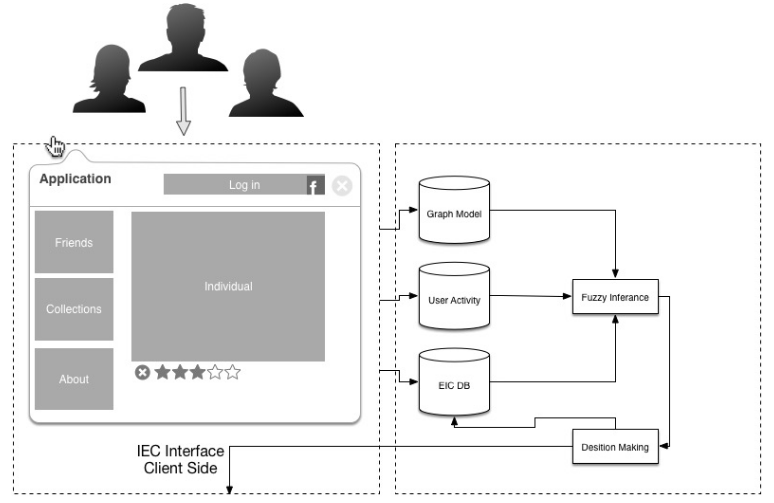
\includegraphics[width=10cm,height=10cm,keepaspectratio]{img/achitecture.png}}
	\caption{Method Architecture.}
	\label{fig:arch}       
\end{figure*}





\section{Graph-based user model} 

To develop a user model, it was necessary to know the factors that are involved in
IEC system. These key factors are the following:

\begin{itemize} 
\item Individuals: The individuals are entities that create the population
of the interactive algorithm.  
\item Users: The users are the entities 
involved in the evaluation of individuals generated in the interactive genetic
algorithm replacing the fitness function.
\item User-Interaction: It is the platform where users make their evaluations in an 
easy and fast way.
\item User activity: They are the set of actions that the user performs in the application. 
\end{itemize}


Knowing these factors a graph-based user modeling is developed. Where the vertices are defined by set of users, individuals, and
collections. The Edges are define by set of relationships as LIKES, KNOWS, HAS, PARENT that represents the relationships between the vertices as seen in \ref{fig:graph}. In this sense a formal definition is given by following definition.


\begin{equation*}\label{eq:graphRelDef} 
\displaystyle 
\begin{split} 
V &= \{[u_1,u_2,u_3,...,u_n],[i_1,i_2,i_3,...,i_n],[c_1,c_2,c_3,...,c_n]\},\\ 
E&= \{[l_1,l_2,l_3,..,l_n],[p_1,p_2,p_3,...,p_n],[h_1,h_2,h_3,...,h_n],[k_1,k_2,k_3,...,k_n]\}\\ 
\end{split} 
\end{equation*} 

Where $V$ is a set of vertices and $u$ represents users, $i$ represents
individuals, and $c$ represents collections. Also $E$ is a set of edges where
$l$ represents the relationship "LIKES" ,$p$ represents the relationship
"PARENT", $h$ represents the relationship "HAS" and finally $k$ that represents
the relationship "KNOWS".

In each vertex is necessary to store some knowledge about them, for instance in
the vertex $u$ has the properties identifier, name, creation date and name type.
Where identifier is a unique number to identifies the user, creation date is a
property where the vertex was created and name type is label for classify the
vertex in this case a “Person” label is apply. Also for vertex $i$ has the
properties identifier,  creation date, name type. Where identifier is a unique
alphanumerical value  that identify the individual, creation date is when this
vertex is created and finally name type that is a label of classify the vertex
in this case a “Individual” label is apply. Now for the  $c$ vertex has the same
properties as the $u$ vertex for their definitions of identifier and creation
date, the difference is the name type property that is a table for classify the
vertex in this case a “Collection” label is apply.

It is important to mention that the application for this research is using
EvoSpace-Interactive through the EvoSpace framework. Also another thing to
mention  is the generation of the initial individual population process in
EvoSpace is gather to transform this individuals in vertices or nodes in order
to  be ready for the evaluations of the users.
 
This user modeling is created when the users starts to interact whith the
application. In order to a user start evaluating individuals  in the application
an essential process is required. These process is that the user has a
“Facebook” account. Ones the user is access he/she can starts to interact with
the different tasks presented by the application. Thus the user can evaluate,
generate collection of individuals and also views friends individuals
collections presented in the human-interacting interface, bring us the creation
of the graph-based user modeling.


\begin{figure*}
\captionsetup{justification=centering,margin=2cm}
\centering
\setlength\fboxsep{0pt}
\setlength\fboxrule{0.7pt}
\fbox{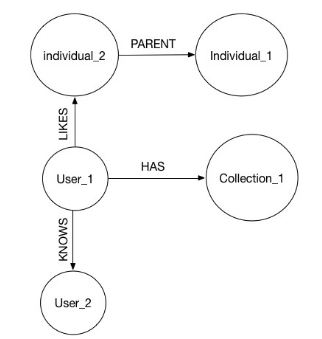
\includegraphics[width=10cm,height=10cm,keepaspectratio]{img/graph.png}}
\caption{GRAPH REPRESENTATION.}
\label{fig:graph}       
\end{figure*}


\section{Interface}
In particular, we shall explain how it was necessary to create an application called “EvoDrawings” to improve the way users interact “collaborate” with an interactive evolutionary computing system. One important class of this application is the user interface, which is the model we will explain in this chapter.

EvoDrawings is a web-based application of interactive evolutionary computing system. In these days when social media platforms has become the perfect tool for masses to exchange information/ideas, interests and creations, EvoDrawings include as a common requirement to the users to have an account of the social platform “Facebook” to have access to the application and consequently participate in it.

The main point to have users logged in the application is that they can evaluate individuals that are formed as a digital paint composed for a single chromosome of nine positions of real numbers.
Each post of the chromosome represents some figure, color, performing behavior, etc. In figure \ref{fig:graph} we can observe a chromosome composed of 15 elements from a digital paint. Once the individual is shown, the users can proceed to evaluate the individual subjectively. This means that according to the user's preferences the user can print his taste in all the evaluations.
The evaluation method consists of giving the desired rating through an interactive visual component of five stars. The interactive visual component allows the user to select from one to five stars to evaluate the individual, having the one star as a slightly liking rate and the five stars like a total satisfaction rate. 
The application enables the user to visualize his social network and the personal evaluation of the users from his social net. In addition to this, the users can create collections with the main goal to allow the users to stock the more pleasing digital paints based on his preferences. 
Also, the user interface contains a section called “About” where the application explains to users in a general way what the application is all about.
For users interact with the interactive evolutionary computation system  it was necessary to develop an application which is called “EvoDrawings”. In this point an explanation of the human-computer interface that was used  is given. 

EvoDrawing It is a Web-based application of interactive evolutionary computation. In this application users need an account of the social network platform in particular "Facebook" to access the application and consequently participate. Once users access can evaluate individuals presented as a digital painting that is composed of a chromosome, where its representation is a vector of real numbers of fifteen positions. Each position in the  chromosome  represents some kind of behavior, for instance  the type of figure, movement, color, and so on. Figure \ref{fig:chromosome} chromosome composed of 15 items represent a digital painting is displayed. Once the individual is shown, users come to evaluate in a subjectively way. This means that according to the likes, preferences, and so on., users conduct their evaluations. 

To evaluate individuals, users are presented with a component of visual interaction based on star ratings. This visual component is from one star to five star where  a star means that the user does not like much the painting and five means total satisfaction. Within the applications users can create collections in order to store paintings are met their expectations, in other words having a grate like for them. 

Users can view their friends who are using the application as well as see what level of experience (participation) in a leaderboard. This in order to motivate them to evaluate more Individuals and consequently Increase Their participation Within the application.

In the interface there is a section of "About" where he explains to users in a general way that addresses the application of EvoDrawigns. In the interface there is a section of "About" which explains to the  users in a breve way what the application is all about. This human-computer web-based interface can be seen in figure x.



\begin{figure*}
\captionsetup{justification=centering,margin=2cm}
\centering
\setlength\fboxsep{0pt}
\setlength\fboxrule{0.7pt}
\fbox{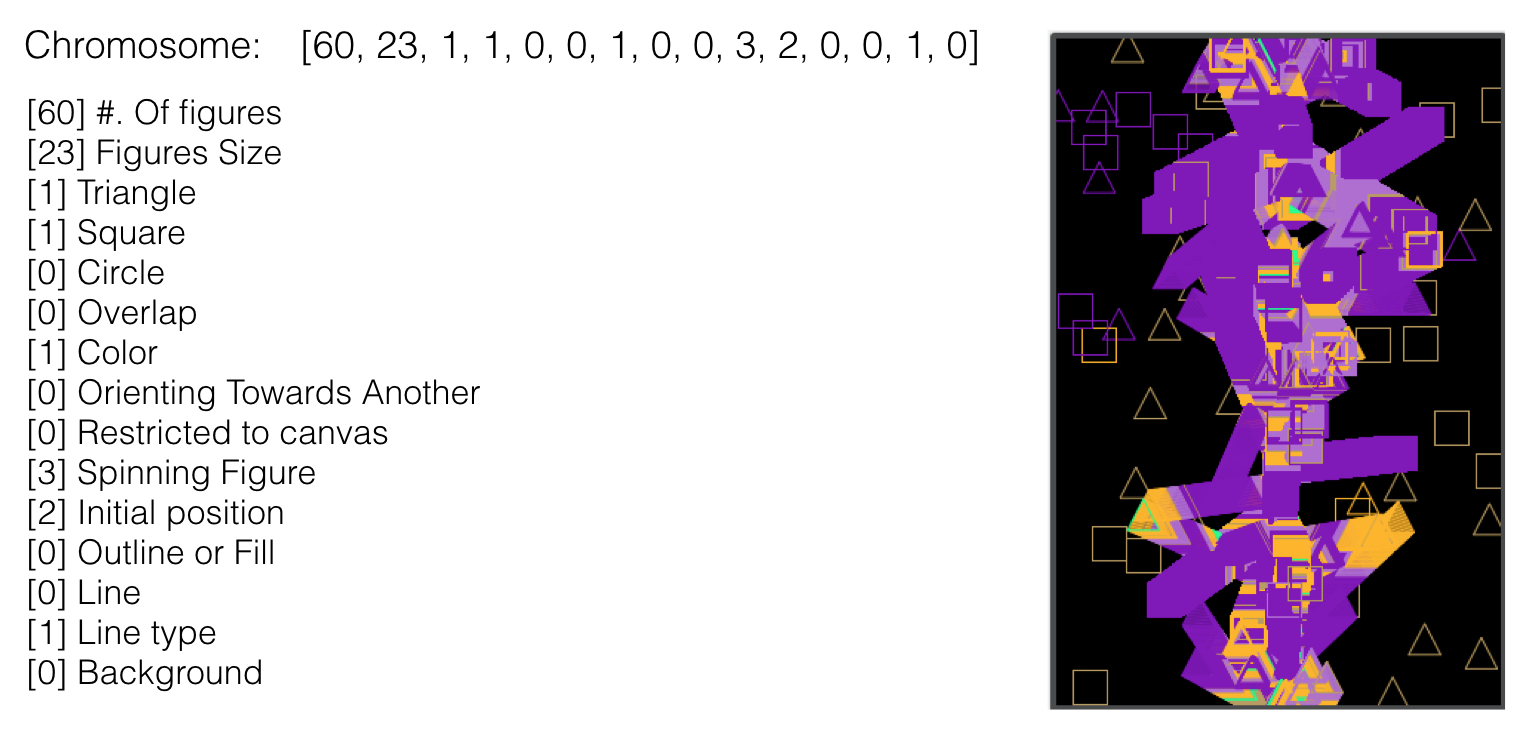
\includegraphics[width=10cm,height=10cm,keepaspectratio]{img/chromosome.png}}
\caption{CHROMOSOME REPRESENTATION.}
\label{fig:chromosome}       
\end{figure*}



We can find the vertices that are defined by the users, individuals, and collections as we can observe in figure 1. The users has the following properties:

\section{User activity}
The user activity is not so different from how the graph is formed, with the difference that the information generated is formed using the standard specified by "JSON activity stream 1.0," which is stored in the engine database NoSQL "Redis ."

An activity consists of 4 elements: an actor, a verb, an object and a target. The activity generates the history of a user and performs an action on an object. For example - "Christian likes the individual 3" or "Mario created a collection". In most cases, the components will be explicit, but may also be implicit.

The primary goal of this specification is to provide sufficient metadata about the activity, to help the consumer of these data to present the information to the user, in a straightforward and user-friendly format. This involves building simple sentences on the activity that is happening, as well as the visual representation of the activity.

So far, we can say that an "Activity Stream" is a collection of one or more activities of an individual (user).
This specification does not define the relations between the activity within the collection, therefore remains to the interpretation of the user who implements it.

\section{Database for interactive evolutionary computation}
Our data store for interactive evolutionary computation consists of two databases, as figure \ref{fig:databases} shown. On one hand one  data base  engine for EvoSpace uses Redis database already explained in Chapter x.  This database contains the structure of individual-user data, where every user participation is store, for instance the fitness of the individual, the  user identifier, the representation of the chromosome, and so on. It is necessary to have this information because is used in the fuzzy inference block , which is explained later in this chapter. 
On the other hand there is a relational database, where basic user information is stored, such as a user ID, your email, user session. Also this database  stores everything needed to meet the requirements process login "Facebook". It also contains the structure for storing collections as shown in Figure ref{fig:databases}.

\begin{figure*}
\captionsetup{justification=centering,margin=2cm}
\centering
\setlength\fboxsep{0pt}
\setlength\fboxrule{0.7pt}
\fbox{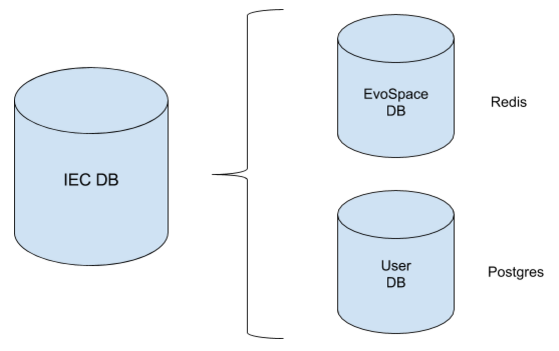
\includegraphics[width=10cm,height=10cm,keepaspectratio]{img/databases.png}}
\caption{DATABASES FOR IEC.}
\label{fig:databases}       
\end{figure*}



The database for interactive evolutionary computation consists of two databases, as we observe in figure X. In one hand we have the EvoSpace database that uses Redis database engine that is already explained in Chapter X section X.

This database contains the structure of individual user data, where every user participation is being stored as well as the fitness of the individual, the user identifier, the representation of the chromosome, etc. 

It is necessary to have this information because it is used for fuzzy inference block, which is explained in another chapter. On the other hand, we have a relational database, where basic user information is stored, such the ID, the email, the session, etc. This database also stores everything needed to meet the requirements of login for "Facebook". One important additional information is that contains the structure for storing collections as we can see in Figure X.

\section{Fuzzy Inference}
In this chapter, we will focus on the explanation of fuzzy inference block. This block uses fuzzy inference to acquire a parameter having the weight function to adjust the participation in interactive evolutionary computing applications. This parameter is used in the decision block which will be explained later in this chapter. Additionally, the parameter is also acquired from the information generated in different databases.

The fuzzy inference system is Mamdani type and is composed of three inputs and one output. Where entries are defined by the preference variable that is also composed of three functions of triangular membership; these features are called low, medium, high, and have ranged from 1 to 5. This range is given by the preference that the user assigns to the individual at the time of assessment.

We also consider the input variable called "experience" and it is defined by three functions of triangular membership under the name of low, medium and high in a range of 1 to 100. The range of this variable are acquired from the activities that the user performs in the application, and empirically with each activity, a score is assigned. For example, if the user makes a login, a three-point score is assigned, as well if the user evaluates an individual, a two-point score is assigned, all the activities has a score punctuation and also the user has a score limit of one hundred points.

The third variable which is called “ranking” it is also defined by three triangular membership functions with the name of low, medium, high, in a range of 1 to 30. This range is defined by a ranking process as well as is also performed in video games; the range is adjusted according to the user participation.

This involvement is acquired from all the cardinality of the graph that the user has and passes through the logarithmic equation X that calculates the value of ranking. Finally, the exit "fuzzyrate" is in a range of 1 to 100 defined by three triangular membership functions with the name of bad, normal and good. In figure ref{fig:Fuzzy} shows this fuzzy inference system.


\begin{enumerate} 

\item \textit{If \textbf{preference} is low and 
\textbf{experience} is low and \textbf{ranking} is low then \textbf{fuzzy-rate} is bad.}
\item \textit{If \textbf{preference} is low and 
\textbf{experience} is low and \textbf{ranking} is mid then \textbf{fuzzy-rate} is bad.}
\item \textit{If \textbf{preference} is low and 
\textbf{experience} is low and \textbf{ranking} is high then \textbf{fuzzy-rate} is bad.}
\item \textit{If \textbf{preference} is low and 
\textbf{experience} is mid and \textbf{ranking} is low then \textbf{fuzzy-rate} is bad.}
\item \textit{If \textbf{preference} is low and 
\textbf{experience} is mid and \textbf{ranking} is mid then \textbf{fuzzy-rate} is bad.}
\item \textit{If \textbf{preference} is low and 
\textbf{experience} is mid and \textbf{ranking} is high then \textbf{fuzzy-rate} is normal.}
\item \textit{If \textbf{preference} is low and 
\textbf{experience} is high and \textbf{ranking} is low then \textbf{fuzzy-rate} is normal.}
\item \textit{If \textbf{preference} is low and 
\textbf{experience} is high and \textbf{ranking} is mid then \textbf{fuzzy-rate} is normal.}
\item \textit{If \textbf{preference} is low and 
\textbf{experience} is high and \textbf{ranking} is high then \textbf{fuzzy-rate} is normal.}
\item \textit{If \textbf{preference} is mid and 
\textbf{experience} is low and \textbf{ranking} is low then \textbf{fuzzy-rate} is bad.}
\item \textit{If \textbf{preference} is mid and 
\textbf{experience} is low and \textbf{ranking} is mid then \textbf{fuzzy-rate} is normal.}
\item \textit{If \textbf{preference} is mid and 
\textbf{experience} is low and \textbf{ranking} is high then \textbf{fuzzy-rate} is normal.}
\item \textit{If \textbf{preference} is mid and 
\textbf{experience} is mid and \textbf{ranking} is low then \textbf{fuzzy-rate} is normal.}
\item \textit{If \textbf{preference} is mid and 
\textbf{experience} is mid and \textbf{ranking} is mid then \textbf{fuzzy-rate} is normal.}
\item \textit{If \textbf{preference} is mid and 
\textbf{experience} is mid and \textbf{ranking} is high then \textbf{fuzzy-rate} is normal.}
\item \textit{If \textbf{preference} is mid and 
\textbf{experience} is high and \textbf{ranking} is low then \textbf{fuzzy-rate} is normal.}
\item \textit{If \textbf{preference} is mid and 
\textbf{experience} is high and \textbf{ranking} is mid then \textbf{fuzzy-rate} is normal.}
\item \textit{If \textbf{preference} is mid and 
\textbf{experience} is high and \textbf{ranking} is high then \textbf{fuzzy-rate} is normal.}
\item \textit{If \textbf{preference} is high and 
\textbf{experience} is low and \textbf{ranking} is low then \textbf{fuzzy-rate} is normal.}\
\item \textit{If \textbf{preference} is high and 
\textbf{experience} is low and \textbf{ranking} is mid then \textbf{fuzzy-rate} is normal.}\
\item \textit{If \textbf{preference} is high and 
\textbf{experience} is low and \textbf{ranking} is high then \textbf{fuzzy-rate} is good.}\
\item \textit{If \textbf{preference} is high and 
\textbf{experience} is mid and \textbf{ranking} is low then \textbf{fuzzy-rate} is normal.}\
\item \textit{If \textbf{preference} is high and 
\textbf{experience} is mid and \textbf{ranking} is mid then \textbf{fuzzy-rate} is normal.}\
\item \textit{If \textbf{preference} is high and 
\textbf{experience} is mid and \textbf{ranking} is high then \textbf{fuzzy-rate} is good.}\
\item \textit{If \textbf{preference} is high and 
\textbf{experience} is high and \textbf{ranking} is low then \textbf{fuzzy-rate} is good.}\
\item \textit{If \textbf{preference} is high and 
\textbf{experience} is high and \textbf{ranking} is mid then \textbf{fuzzy-rate} is good.}\
\item \textit{If \textbf{preference} is high and 
\textbf{experience} is high and \textbf{ranking} is high then \textbf{fuzzy-rate} is good.}\

\end{enumerate} 

\begin{figure*}
\captionsetup{justification=centering,margin=2cm}
\centering
\setlength\fboxsep{0pt}
\setlength\fboxrule{0.7pt}
\fbox{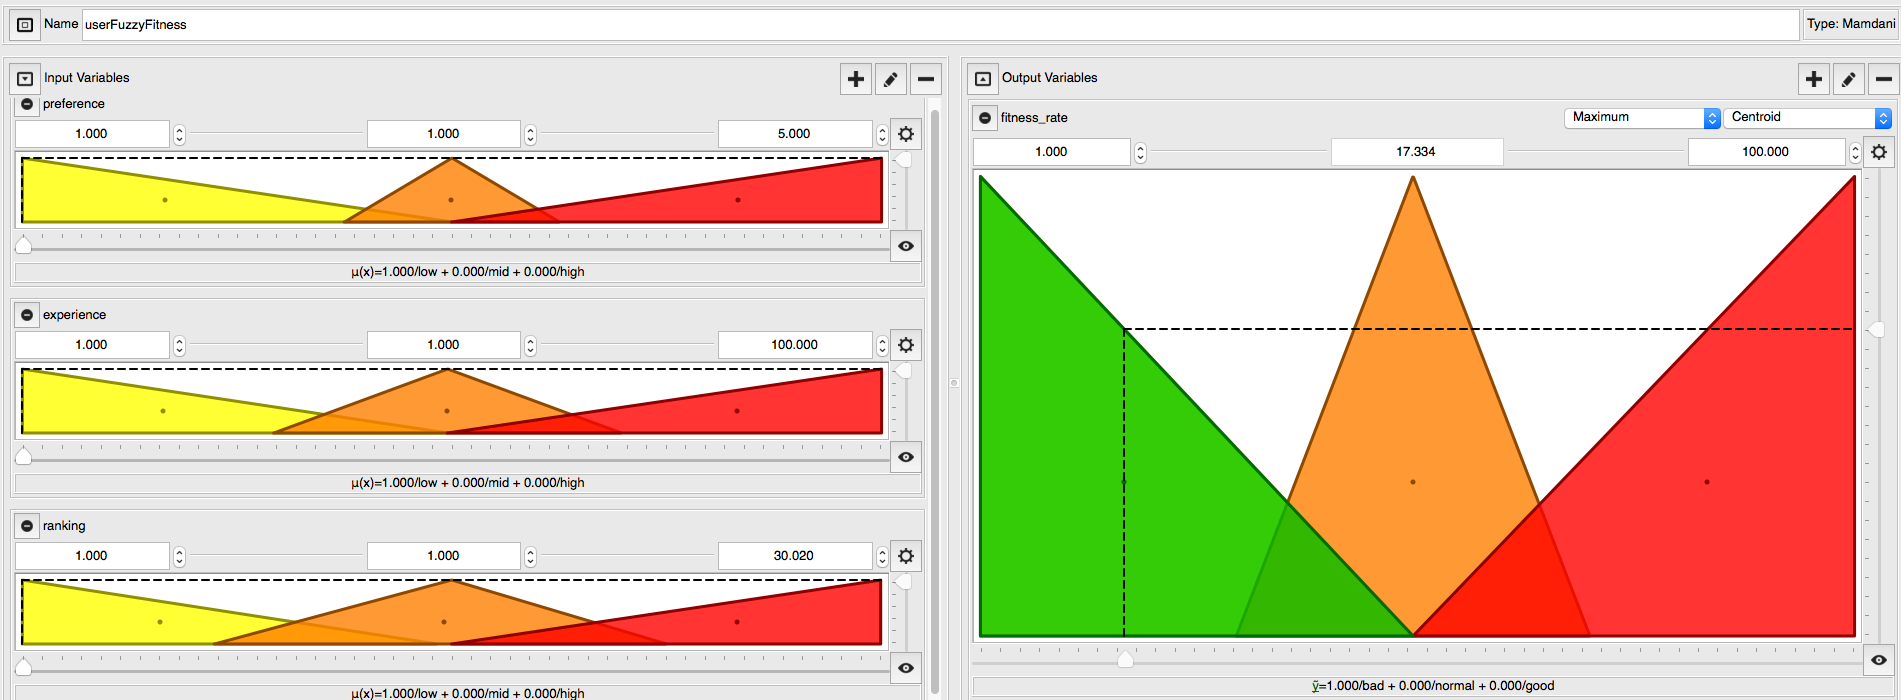
\includegraphics[width=10cm,height=15cm,keepaspectratio]{img/fuzzySys.png}}
\caption{Fuzzy Inference System.}
\label{fig:Fuzzy}       
\end{figure*}


\section{Decision Making}
The decision block it is defined by equation \ref{eq:fuzzyfitness} representing the value of fitness that takes the individual to be evaluated by the user, as well as everything else that makes in the application.

\begin{equation}\label{eq:fuzzyfitness}
\displaystyle f(ff)=\frac{\sum_{i=0}^{n}x_{i}f(y_{i})}{\sum_{i=0}^{n}f(y_{i})}
\end{equation}

Where  $ff$ represents the fuzzy fitness function for all users who have evaluated an individual of the population in particular.
Likewise $x$ represents the range that a user assigned to the individual according to their preferences, likes, and so on. The function $f(y_i)$ represents the fuzzy inference and is defined by the equation \ref{eq:fuzzyInference}.

\begin{equation}\label{eq:fuzzyInference}
\displaystyle f(y_i)= fr(x, e, r)
\end{equation}

Where $x$ is still the range that users assigned to a particular individual. The variable $e$represents the user experience, which is a function that is defined in equation \ref{eq:fuzzyInference}.

\begin{equation}\label{eq:userEperience}
\displaystyle f(e) = \sum_{i=0}^{n}l_{i}j_{i}s_{i}s_{i}
\end{equation}

Where $i$ represents user activity. The variable $l$ represents the taste generated of the verb "like" from the user activity stream.
The variable  $j$ represents the access that like the variable  is obtained from the verb "join" from the user activity stream. The variables $s, o$ are represented by the verbs "save" and "open" from the user activity stream.

\begin{equation}\label{eq:scale}
\displaystyle s =\frac{levels}{log_{2}fp}
\end{equation}

In equation \ref{eq:fuzzyInference}, we can find the variable $r$ as the last parameter of the function and represents a ranking of the user; this variable is defined by a logarithmic scale where intervenes our graph-base user modeling  and is defined by Equation \ref{eq:scale}.

In equation \ref{eq:scale}, the variable $s$ represents the scale and $levels$ represents the highest level that the users can have. The variable $fp$ represents the final points, which are the maximum points that a particular user can have.

In order to acquire the user's ranking level , a floor function  is calculated, the main point of this is to increase the difficulty for the high ranked users to level up. In other words the expert users needs to have more participation if they want to increase their level ranking. This function is defined by equation \ref{eq:floorf}.

\begin{equation}\label{eq:floorf}
\displaystyle rl=\lfloor(s)(log_2pf)\rfloor
\end{equation}

Where $rl$ represents the ranking level, $s$ represents the scale and  are all the participations  that the user has made. These participations represents the degree that the user has within his own graph and is defined by the vicinity of its vertex  that is given by the adjacent vertices to $u$, defined in Equation \ref{eq:neighbors}.

\begin{equation}\label{eq:neighbors}
\displaystyle N(u)={\{y\in V_{G}|\{u,y}\in E_{G}\}
\end{equation}

In this case the degree of the vertex $u$ is the number of neighbors of: 

\begin{equation}\label{eq:degree}
\displaystyle g(u)=|N(x)|
\end{equation}












\chapter{Case study} \label{sec:4}




\section{Motivation and objectives}

Our motivation begins to know if a user model in combination with
other techniques such as usability or fuzzy logic increases the participation of users in a
given Web-based IEC application. It is well know that one of the main
problems in these systems is fatigue, who is the cause by the large 
amount of individual evaluations
that the user need to preform and consequently their participation decreases.

Our approach goes with the sense of increasing the participation of the users
within these applications, providing to them very simple tasks to execute in order to
capture their attention as well as to know their behavior.


Since we have described that the main approach is to increase the participation
of users, in order to measure these results and to be able to demonstrate 
if the participation 
of these users increase, it was necessary to build a study
case where an evolutionary art application is involved within an interactive
evolutionary system which we call EvoDrawings. This application was modified in
order to obtain three versions of this one, which were labeled with the names
ED01, ED02, ED03. The objective is to extract data from each of the different
versions and then quantify and compare which of these had the best result in the
participation of the users.

\section{EvoDrawings} EvoDrawings is based on the EvoSpace-i framework and
consequently uses the same architecture which is presented in figure
\ref{fig:ESFramework}. This architecture have the individual block which
contains different information, including the chromosome that represents the
digital painting. Technically the individual is an associative arrangement
(dictionary) where an abstract collection of keys and values is stored with a
one-to-one association. Where keys represent a specific property in each object
and the values are different types of data, such as lists, tuples, numbers,
strings and dictionaries.

\begin{figure*}
\captionsetup{justification=centering,margin=2cm}
\centering
\setlength\fboxsep{0pt}
\setlength\fboxrule{0.7pt}
\fbox{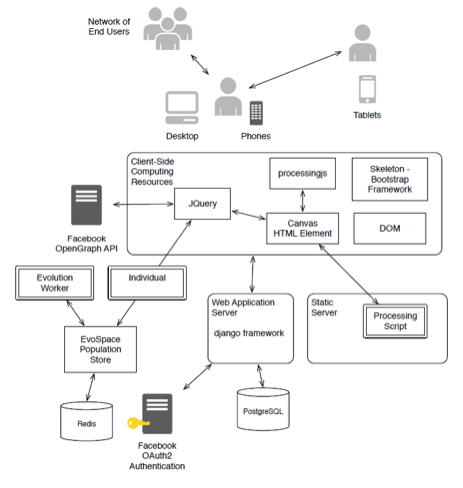
\includegraphics[width=8cm,height=8cm,keepaspectratio]{img/ESFramework.png}}
\caption{EvoSpace-i framework.}
\label{fig:ESFramework}
\end{figure*}


The individual has the following fields, shown in figure \ref{fig:individual_dic}.
The field is represented by a single string for each object. The chromosome
field represented by a string, which for EvoDrawing represents an array of 15
numerical characters which define the behavior of the digital drawing. The
fitness field is defined by a dictionary, this field contains the information of
users evaluations as well as the creation date as a timestamp. The field called
views is determined by a string and represent the number of times they have seen
the individual. The keys called mom and dad define where the individual comes
from. The GeneticOperator field is a string that specifies the genetic operator
produced.

\begin{figure*}
\captionsetup{justification=centering,margin=2cm}
\centering
\setlength\fboxsep{0pt}
\setlength\fboxrule{0.7pt}
\fbox{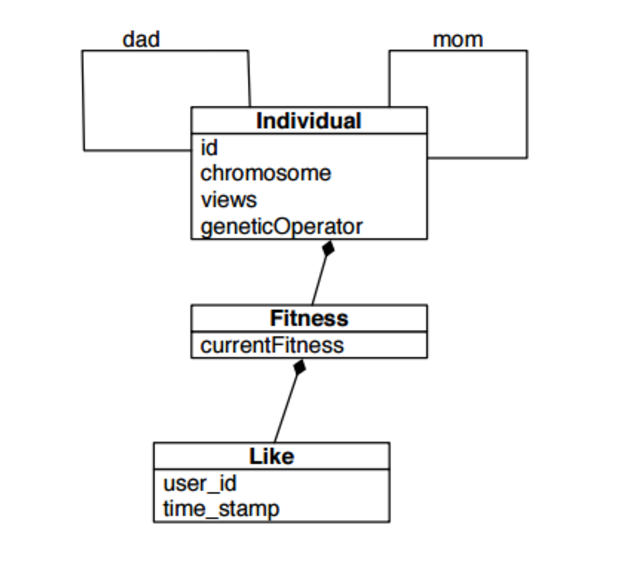
\includegraphics[width=8cm,height=8cm,keepaspectratio]{img/individual_dic.png}}
\caption{Chromosome representation.}
\label{fig:individual_dic}
\end{figure*}

\subsection{Processing Script}
It is necessary to explain how the animation
that the users visualize works. EvoSpace-i uses processing script in order to do
the rendering of the individuals which contain the behavior of the figures. This
application can run in browsers that are compatible with HTML 5, this is due to
the use of a JavaScript library called processingscriptjs that is in charge of
communicating with the base script and thus perform the render on HTML 5 canvas
in The EvoDrawings application.

\subsection{Fitness}
The fitness assignment for each individual is given by the
evaluations of users. EvoDrawings has reviews when users give their
rating. We can see this rating on figure x of the %Figure x?? - Mario
interface that EvoDrawings uses in all its variations. This rate ranges from 1
star to 5 stars, which defines the user's liking for the digital drawing
presented by EvoDrawings. When users evaluate a sample of individuals, some of
these will not receive any evaluation. The view property, it increases by 1 when
it is viewed. Internally, a fitness calculation is used defined by the following
equation:

\begin{equation}\label{eq:fitfunc01}
\displaystyle fitness=\frac{\sum_{i=0}^{n}x_{i}+ 1}{\sum_{i=0}^{n}v_{i} + 1}
\end{equation}

$i$ represents the individual's.
$x$ is the range that individuals received when evaluated by users.
$v$ are the views that users have viewed individuals.

The above is used in version ED01. For the next two versions we use a different
defined fitness based on the behavior that users perform within EvoDrawings,
such as assigned tasks, the logging action in order to start evaluating
individuals, individuals evaluation, creating collections for later store
individuals and finally view the public individuals of friends who are
participating in the application.

For ED02 we use a fuzzy inference system consisting of two inputs and one
output. Entries are defined by preference and experience. The preference is the
range of stars from 1 to 5 and are the evaluations that users give to the
presented digital drawing, and are represented with triangular membership
functions called high, medium and low. In the same way the input experience is
defined by the tasks performed and it has the range of 1 to 100, each task
receives points until reaching a threshold of 100 points where the user is
considered as an expert within the application. This input is also represented
by triangular membership functions called high, medium, low. Finally we have the
output called fuzzy\_rate in a range of 1 to 100, defined by triangular
membership functions called bad, normal, good. This fuzzy system consists of 9
if-then rules:

\begin{enumerate}
	\item \textit{If \textbf{preference} is low and
		\textbf{experience} is low then \textbf{fuzzy\_rate} is bad.}
	\item \textit{If \textbf{preference} is mid and
		\textbf{experience} is low  then \textbf{fuzzy\_rate} is bad.}
	\item \textit{If \textbf{preference} is high and
		\textbf{experience} is low  then \textbf{fuzzy\_rate} is normal.}
	\item \textit{If \textbf{preference} is low and
		\textbf{experience} is mid then \textbf{fuzzy\_rate} is bad.}
	\item \textit{If \textbf{preference} is mid and
		\textbf{experience} is mid  then \textbf{fuzzy\_rate} is normal.}
	\item \textit{If \textbf{preference} is high and
		\textbf{experience} is mid  then \textbf{fuzzy\_rate} is good.}
	\item \textit{If \textbf{preference} is low and
		\textbf{experience} is high then \textbf{fuzzy\_rate} is normal.}
	\item \textit{If \textbf{preference} is mid and
		\textbf{experience} is high  then \textbf{fuzzy\_rate} is good.}
	\item \textit{If \textbf{preference} is high and
		\textbf{experience} is high  then \textbf{fuzzy\_rate} is good.}

\end{enumerate}

The fitness function is given by the following equation:

\begin{equation}\label{eq:fitfunc02}
\displaystyle fitness=\frac{\sum_{i=0}^{n}x_{i}+f(y_{i})}{\sum_{i=0}^{n}f(y_{i})}
\end{equation}

$i$ represents the individual's. x is the range that users give to individuals..
$f(y_i)$ represents a fuzzy function composed of a fuzzy inference system and is
represented by the equation \ref{eq:fuzzyFunc}.

\begin{equation}\label{eq:fuzzyFunc}
\displaystyle y=fr(x,e)
\end{equation}


$fr$ represents the fuzzy rate. $x$ it remains the range that users give
according to their preferences to individuals. $e$  is the experience that is
defined by the activity that the user is doing within the application. The fuzzy
inference system of it is a Mamdani type composed of two inputs that are  $x,e$
and a fuzzy rate output as shown in figure \ref{fig:fis_01}.

\begin{figure*}
\captionsetup{justification=centering,margin=2cm}
\centering
\setlength\fboxsep{0pt}
\setlength\fboxrule{0.7pt}
\fbox{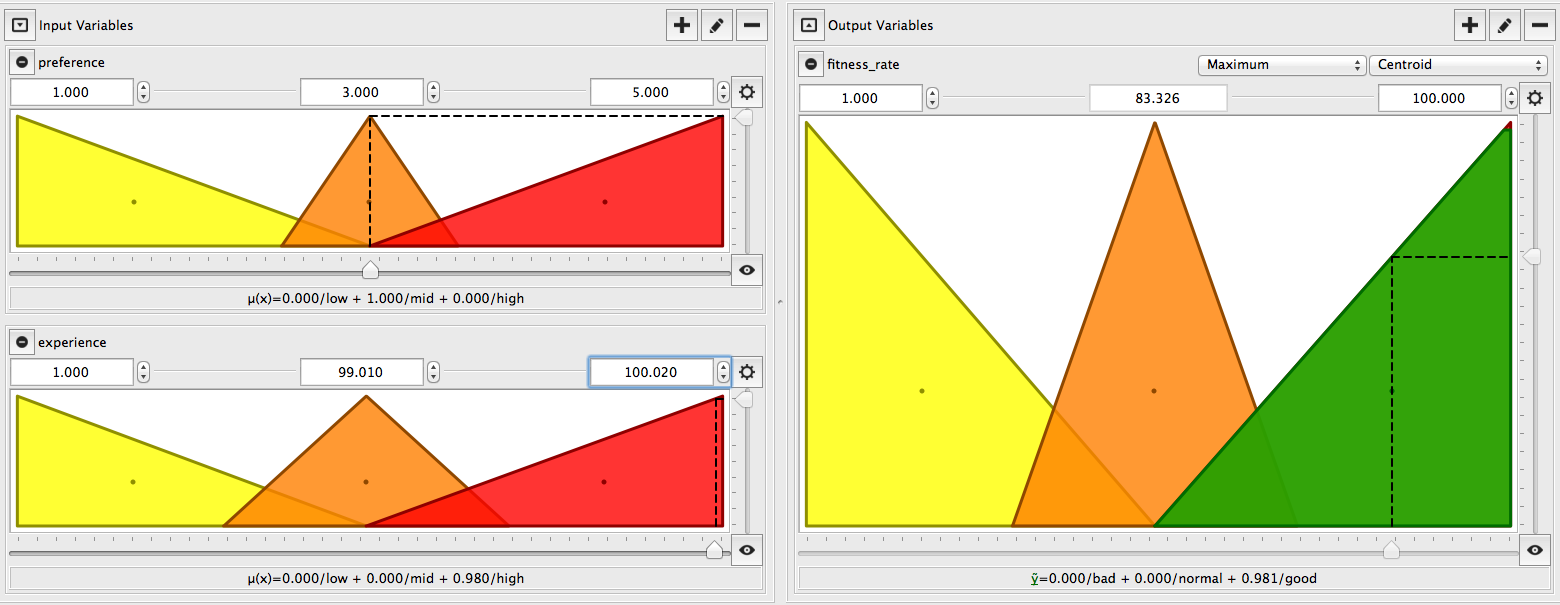
\includegraphics[width=12cm,height=10cm,keepaspectratio]{img/fuzzy_system_2_1.png}}
\caption{Chromosome representation.}
\label{fig:fis_01}
\end{figure*}

For ED03 the fitness function is given by the same equation as ED02 the
difference relies in the inputs of the fuzzy function, for this case a new input
is added with the name of ranking. This new input is the given by the
cardinality of the graph of the user model for each user. here is the fuzzy
function for ED03.

\begin{equation}\label{eq:fuzzyFunc2}
\displaystyle y=fr(x,e,r)
\end{equation}

$fr$ represents the fuzzy rate.
$x$ it remains the range that users give according to their preferences to individuals.
$e$  is the experience that is defined by the
activity that the user is doing within the application.
$r$ is the ranking the user within the graph model.
 The fuzzy inference system it is a Mamdani type composed of three inputs that
are  $x,e, r$ and a fuzzy rate output as shown in figure \ref{fig:fis_02}.

\begin{figure*}
\captionsetup{justification=centering,margin=2cm}
\centering
\setlength\fboxsep{0pt}
\setlength\fboxrule{0.7pt}
\fbox{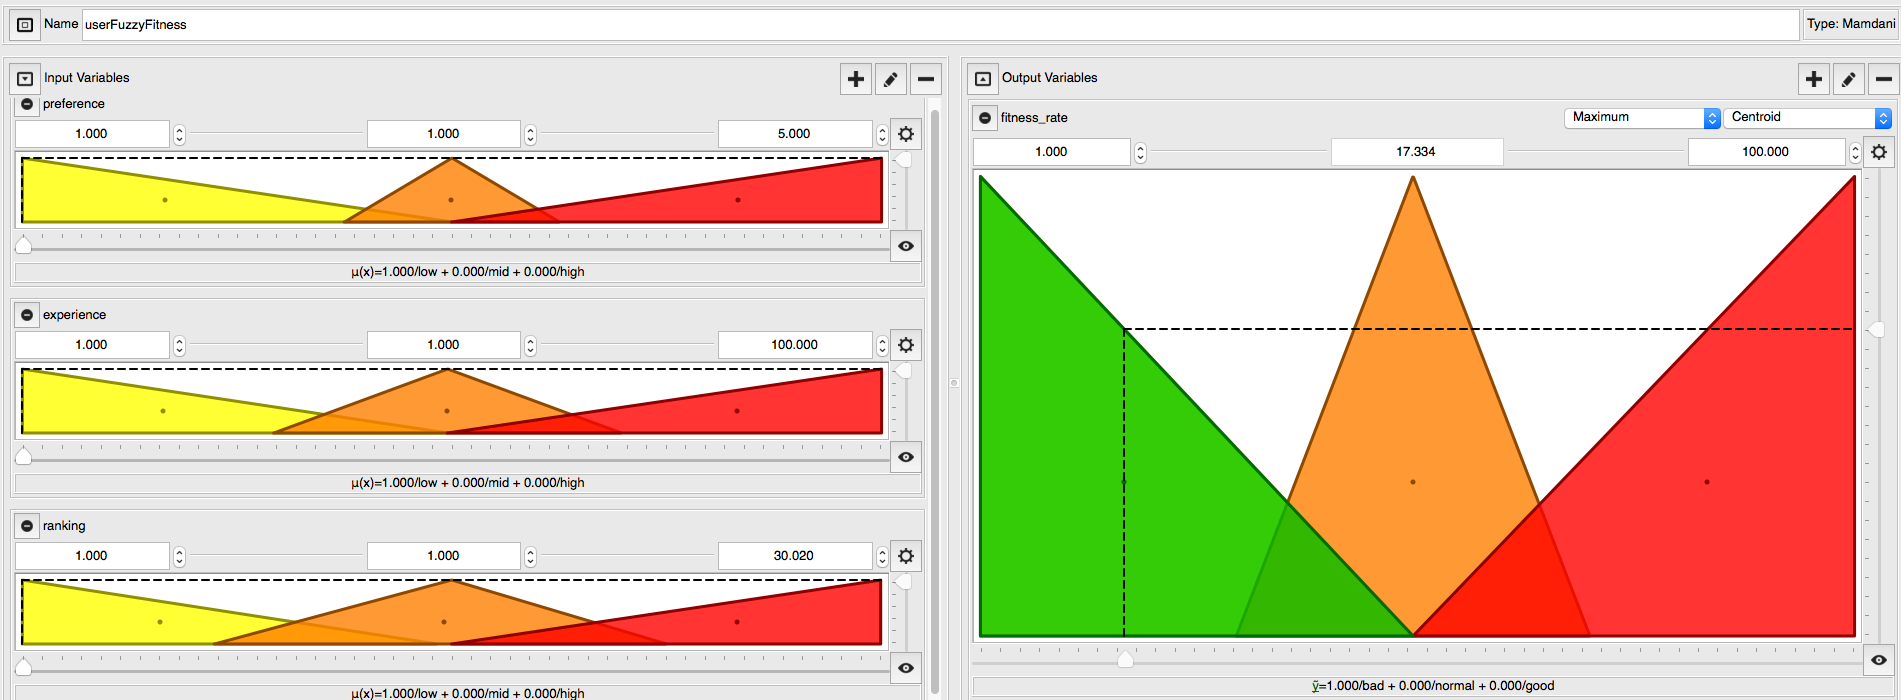
\includegraphics[width=12cm,height=10cm,keepaspectratio]{img/fuzzySys.png}}
\caption{Fuzzy inference system for ED03.}
\label{fig:fis_02}
\end{figure*}


\subsection{Configurations.}

Previously we mentioned that EvoDrawings is an application of evolutionary art
within an evolutionary system with the aim of being able to prove the increase
of the participation of the users. To prove this hypothesis within this thesis,
3 different versions of EvoDrawing were designed. The EvoDrawing versions and
the results of the experiments were compared to each other. All experiments and
comparisons were performed on equal data, parameters and users.

For ED03 the initial configuration of our evolutionary algorithm in this version
is the following:

\begin{enumerate}
	\item  \textbf{We have an initial population of 80 individuals.}

	\item  \textbf{An evolution parameter is 8 evaluations.}

	\item  \textbf{A mutation parameter of }
	\item  \textbf{With random selection between competition.}
	\item  \textbf{One horizontal genetic crossing Operator.}
	\item  \textbf{The fitness is given by the equation \ref{eq:fitfunc01}.}
\end{enumerate}

For the interface in this version there is an easy-to-use Web interface for
users to evaluate  individuals. Figure\ref{fig:UI_01} shows the navigation
bar that has the functionality for logging in to the application.
Once logged in with a Facebook account, an avatar appears in the navigation bar
as well as the functionality to exit the application through a logout button. Also
within this interface exists the visual element \'Friends\' where all the friends
that are participating in the application appear, this element also has the
functionality to be able to see the public collections that the these friends have.
Continuing with the explanation of the interface we have the \'Collections\' panel
which shows a list of collections that users have created and saved, as well as
the functionality to create new collections. Within this we have
an \'About this\' section where users can read general information about the
system. Users can evaluate individuals throu a
visual canvas element that shows the behavior of the individual subject to
evaluation (animation) and at the bottom is given the ability to evaluate the
individual with a range of stars where one star means the user did not like it
very much and five stars mean the user like it too much. Now at the bottom of
the star range we have a button that provides the functionality of being able to
add this individual to a collection. At
the top of the star rank is a label with the legend that says 'Click here to
see my DNA History' this takes the user to a detail page about the individual that is 
been evaluated, this is shown
in Figure~\ref{fig:dna}.

\begin{figure*}
\captionsetup{justification=centering,margin=2cm}
\centering
\setlength\fboxsep{0pt}
\setlength\fboxrule{0.7pt}
\fbox{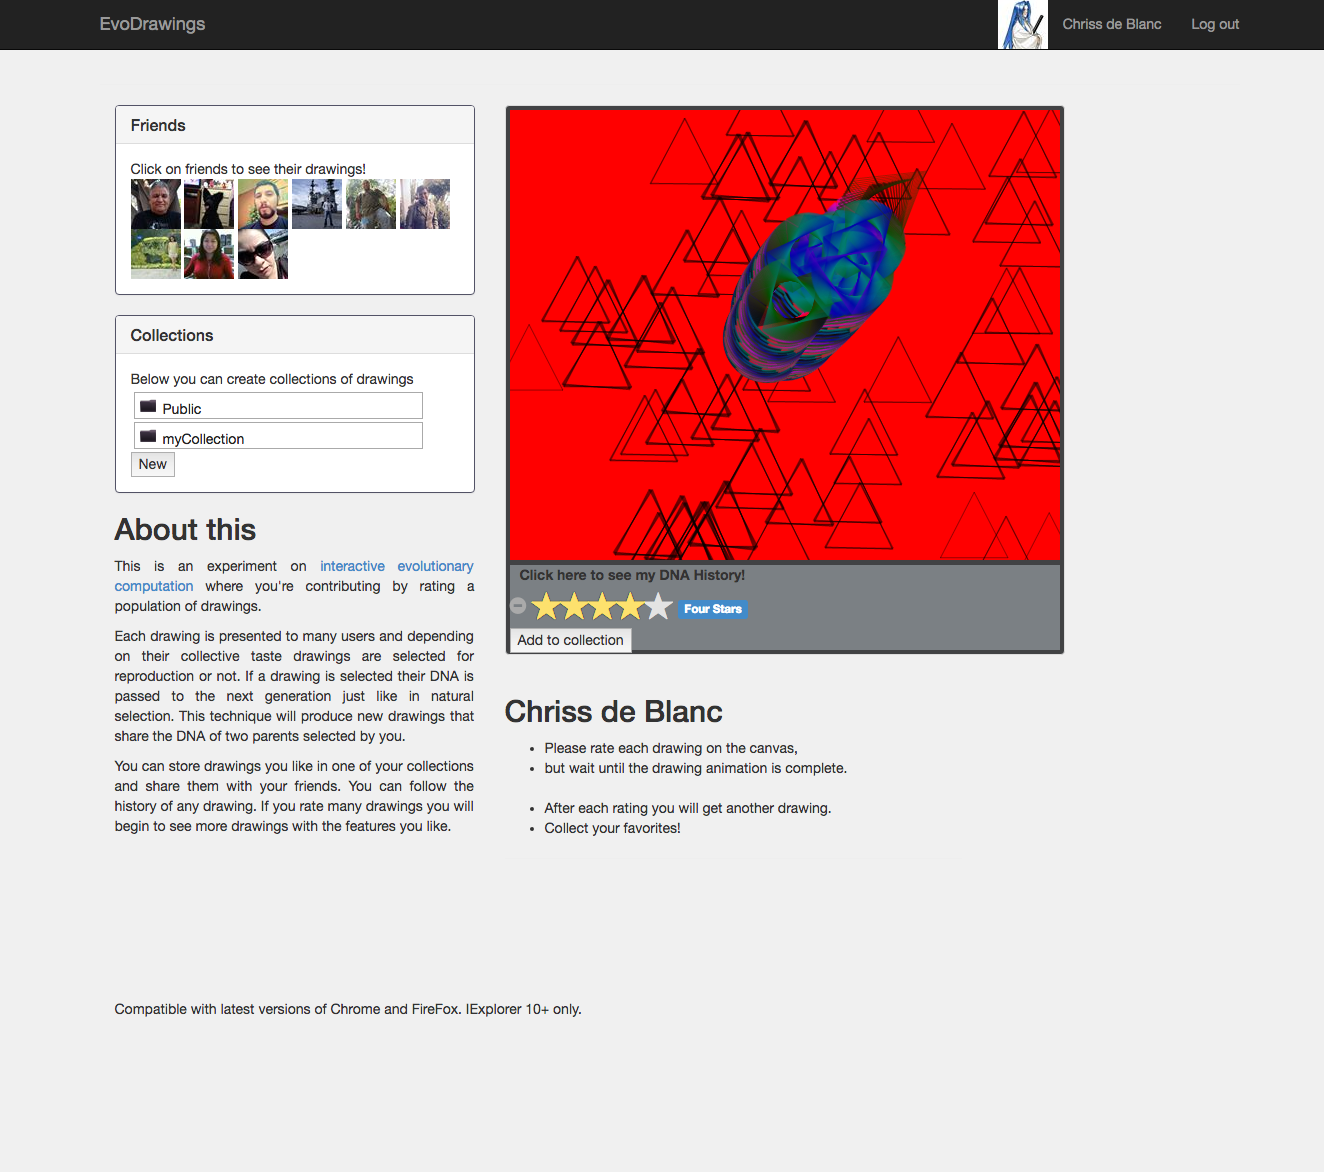
\includegraphics[width=12cm,height=10cm,keepaspectratio]{img/UI_ed01.png}}
\caption{User interface ED01.}
\label{fig:UI_01}
\end{figure*}

This detail presents important information about the individual's DNA history,
such as the number of evaluations he has received in the form of likes, the
number of views as well as the ancestry, his genetic crossing operator, the
numerical representation of his chromosome and its identifier within the
population.



\begin{figure*}
\captionsetup{justification=centering,margin=2cm}
\centering
\setlength\fboxsep{0pt}
\setlength\fboxrule{0.7pt}
\fbox{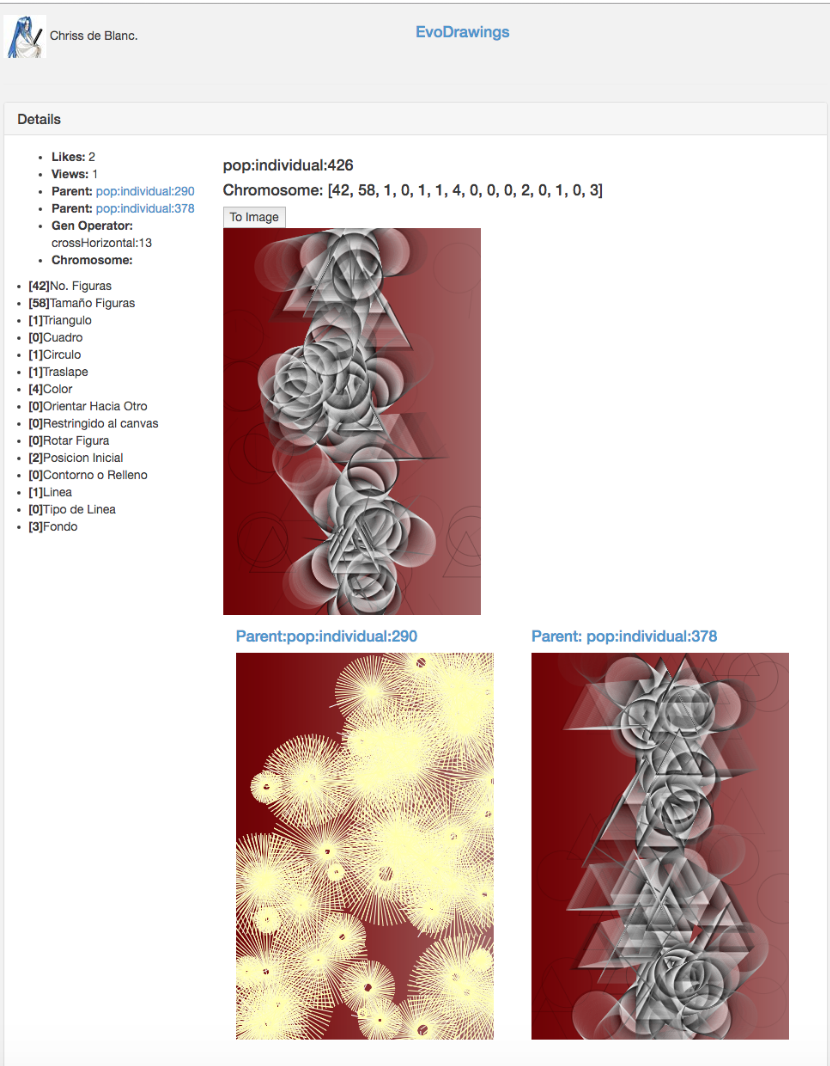
\includegraphics[width=12cm,height=10cm,keepaspectratio]{img/dna.png}}
\caption{DNA history.}
\label{fig:dna}
\end{figure*}

For ED02 there is an initial configuration of the interactive evolution
algorithm as follows:

\begin{enumerate}
	\item  \textbf{We have an initial population of 80 individuals.}

	\item  \textbf{An evolution parameter is 8 evaluations.}

	\item  \textbf{A mutation parameter of }
	\item  \textbf{With random selection between competition.}
	\item  \textbf{One horizontal genetic crossing Operator.}
	\item  \textbf{The fitness is given by the equation \ref{eq:fitfunc02}.}
\end{enumerate}

The user interface of this version is the same as the previous version. The
difference between versions lies in how the inference is made internally.

For ED03 there is an initial configuration of the interactive evolution
algorithm as follows:
\begin{enumerate}
	\item  \textbf{We have an initial population of 80 individuals.}

	\item  \textbf{An evolution parameter is 8 evaluations.}

	\item  \textbf{A mutation parameter of }
	\item  \textbf{With random selection between competition.}
	\item  \textbf{One horizontal genetic crossing Operator.}
	\item  \textbf{The fitness is given by the equation \ref{eq:fitfunc02}.}
\end{enumerate}

This version has a new input on the fuzzy functionality named ranking and this
value is given by the cardinality of the graph by each user within the graph-
based user model. Also the fuzzy inference system has a 27 if-then rules which
can visualize in appendix b. The second difference is the usability elements
where the gamification paradigm is apply. Figure \ref{fig:intarface03} shows this
usability elements that are the score level, the experience level and also the
leader board element.

\begin{figure*}
\captionsetup{justification=centering,margin=2cm}
\centering
\setlength\fboxsep{0pt}
\setlength\fboxrule{0.7pt}
\fbox{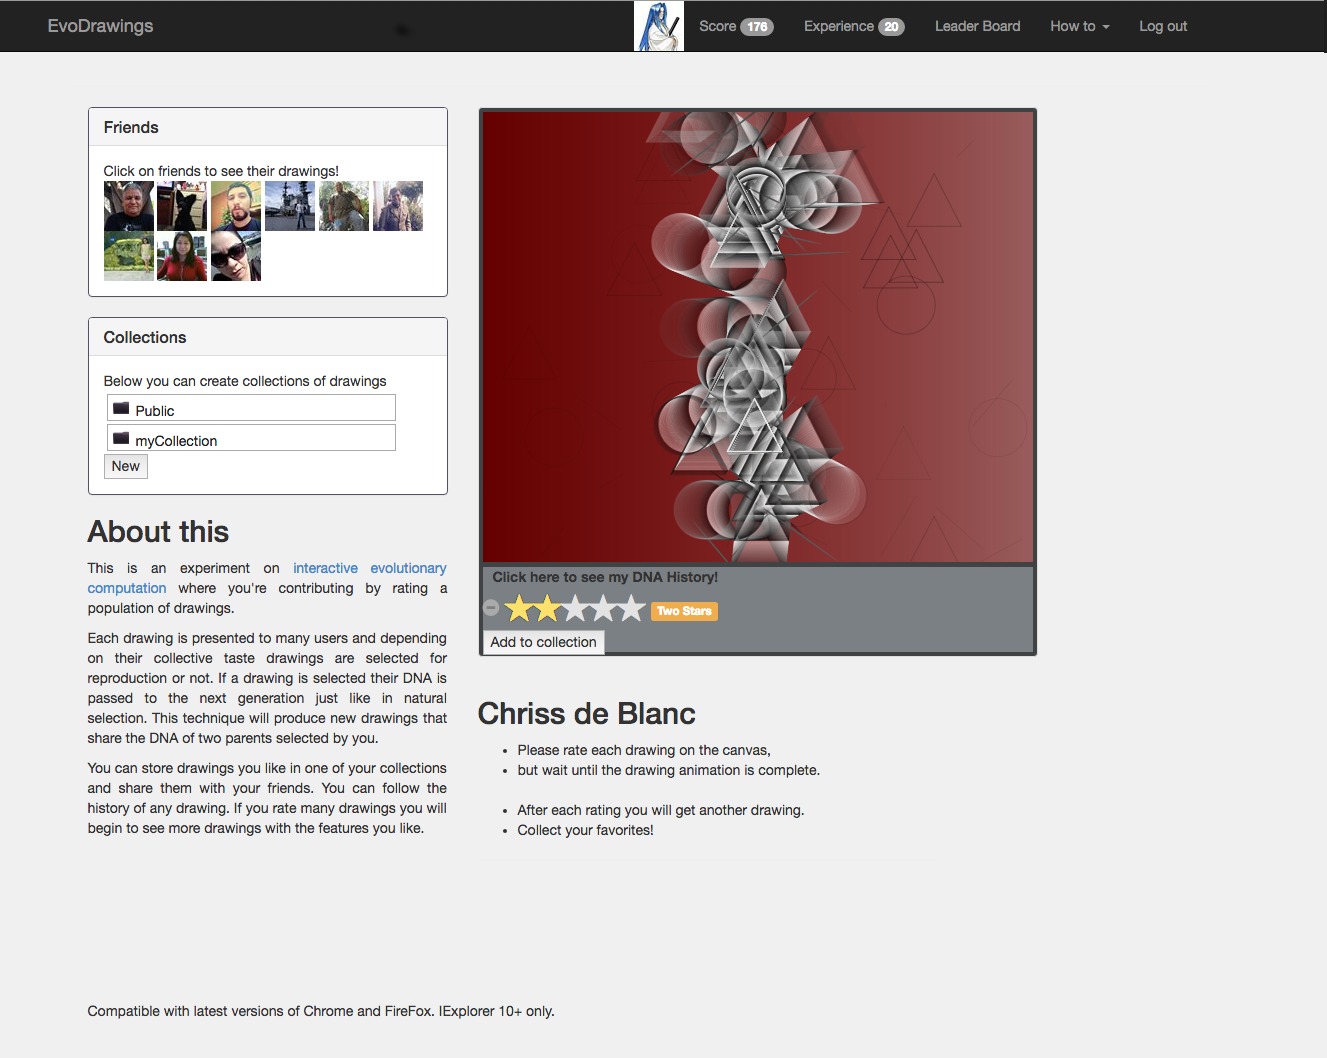
\includegraphics[width=12cm,height=10cm,keepaspectratio]{img/interface.png}}
\caption{ED03 Web interface.}
\label{fig:intarface03}
\end{figure*}

This elements in the navigation bar is for users to visualize their scores
inside ED03 application. Likewise the level of experience that is acquiring
through its participations. This version also has an option to see the table of
leaders within the application as shows in figure \ref{fig:leaderBoard}. This
table shows the 10 best users and the number of entries that have been made so
far.


\begin{figure*}
\captionsetup{justification=centering,margin=2cm}
\centering
\setlength\fboxsep{0pt}
\setlength\fboxrule{0.7pt}
\fbox{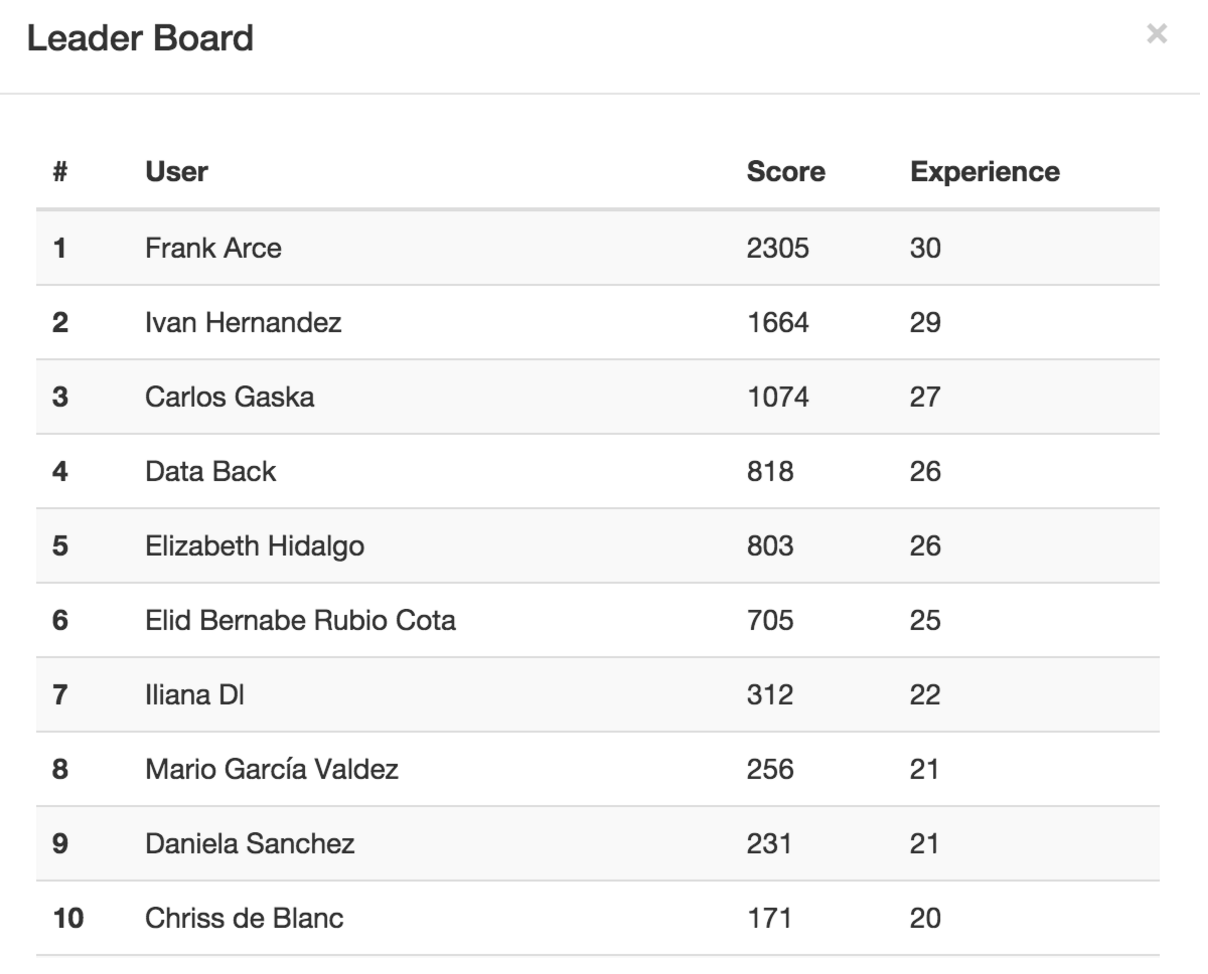
\includegraphics[width=12cm,height=10cm,keepaspectratio]{img/leaderBoard.png}}
\caption{Leader board at ED03.}
\label{fig:leaderBoard}
\end{figure*}


\subsection{Promote.}

Each of the experiments was promoted through social networks particularly on
Facebook and Twitter platforms through a short URL as well as an ad to motivate
users to press the link (short URL). This is in order to find participants on a
voluntary basis. This short URL can be seen in table \ref{tab:PromoteUrl}.

\begin{table}
\small
\caption{Short URL for promoting the applicatins.}
\label{tab:PromoteUrl}
\centering
\small
\begin{tabular}{p{5cm} p{4cm}  }
\hline\noalign{\smallskip}
 Long URL & Short URL \\
\noalign{\smallskip}\hline\noalign{\smallskip}
\small{evodrawings01.herokuapp.com } & \small{goo.gl/J8TCe1}  \\ \hline
\small{evodrawings02.herokuapp.com } & \small{goo.gl/jqjNy5}  \\ \hline
\small{evodrawings03.herokuapp.com} & \small{goo.gl/J8TCe1}  \\ \hline
\noalign{\smallskip}\hline
\end{tabular}
\end{table}


\subsection{Heroku dynos and ad-ons server configurations.}
It is necessary to be mentioned that each of the experiments was implemented
under the cloud service (Heroku), in the following figure \ref{tab:heroku} can
visualize its characteristics by each of the experiments.
\begin{table}
	\small
	\caption{characteristics of  resources and services in cloud Heroku.	}
	\label{tab:heroku}
	\centering
	\small
	\begin{tabular}{p{4cm} p{3cm} p{3cm} p{3cm}  }
		\hline\noalign{\smallskip}
		Service and resources & ED01 & ED02 & ED03 \\
		\noalign{\smallskip}\hline\noalign{\smallskip}
		\small{Heroku Free} & \small{\checkmark} & \small{\checkmark} & \small{\checkmark}\\ \hline
		\small{Deploy from Git} & \small{\checkmark} & \small{\checkmark} & \small{\checkmark}\\ \hline
		\small{Automated patching} & \small{\checkmark} & \small{\checkmark} & \small{\checkmark}\\ \hline
		\small{Self healing apps} & \small{\checkmark} & \small{\checkmark} & \small{\checkmark}\\ \hline
		\small{Undefined logs} & \small{\checkmark} & \small{\checkmark} & \small{\checkmark}\\ \hline
		\small{Number of process types} & \small{2} & \small{2} & \small{2}\\ \hline
		\small{Always on Sleep after 30 mins of inactivity, otherwise always on depending on you remaining mostly free dynes hours} & \small{\checkmark} & \small{\checkmark} & \small{\checkmark}\\ \hline
		\small{Custom domains} & \small{\checkmark} & \small{\checkmark} & \small{\checkmark}\\ \hline
		\small{RAM 512} & \small{\checkmark} & \small{\checkmark} & \small{\checkmark}\\ \hline
		\small{Dedicated} & \small{x} & \small{x} & \small{x}\\ \hline
		\small{Heroku Postgres ::DB Hobby Dev} & \small{\checkmark} & \small{\checkmark} & \small{\checkmark}\\ \hline
		\small{GrapheneDB Chalk} & \small{\checkmark} & \small{x} & \small{\checkmark}\\ \hline
		\small{Redis To Go Nano} & \small{\checkmark} & \small{x} & \small{\checkmark}\\ \hline
		\small{GrapheneDB Sandstone} & \small{x} & \small{x} & \small{\checkmark}\\ \hline
		\small{Redis To Go Mini} & \small{x} & \small{x} & \small{\checkmark}\\ \hline


		\noalign{\smallskip}\hline
	\end{tabular}
\end{table}


The initial purpose of the experiments is to design specific applications and
interfaces to enable users to participate voluntarily within the different
applications. Each experiment allowed the task of collecting data that will
later be analyzed to determine which of these versions had the largest number of
user participations. To verify the initial hypothesis, 3  versions were implemented with 
slight differences in the configuration characteristics of each application, 
which allowed to decide through the results obtained which of them verify the 
hypothesis of this investigation. The results obtained
are presented in the next chapter.

\chapter{Results} \label{sec:6} This chapter presents the results obtained from
the case study discussed in the previous chapter.

\section{EvoDrawing01}

Experiment ED01 generated a user-model graph with the following data
presented(Table\ref{tab:dataGenerated_1}).

\begin{table}
\small
\caption{Data generated in the graph-based user model.}
\label{tab:dataGenerated_1}
\centering
\small
\begin{tabular}{p{3cm} p{3cm} p{3cm} }
\hline\noalign{\smallskip}
  & Data &  \\
\noalign{\smallskip}\hline\noalign{\smallskip}
\small{Nodes} & \small{595} & \\ \hline
\small{Relationships} & \small{2220} & \\ \hline

\noalign{\smallskip}\hline
\end{tabular}
\end{table}


This data is the total of nodes as well as their relationships. Also in
Table~\ref{tab:totalUsers_12} is shown the total of volunteer active users.

\begin{table}
\small
\caption{Total number of volunteers active users.}
\label{tab:totalUsers_12}
\centering
\small
\begin{tabular}{p{3cm} p{3cm} p{3cm} }
\hline\noalign{\smallskip}
  & Users &  \\
\noalign{\smallskip}\hline\noalign{\smallskip}
\small{Total } & \small{53} & \\ \hline
\noalign{\smallskip}\hline
\end{tabular}
\end{table}

In order to observe which users have better social interconnectivity within the
experiments it was decided to make a relation of number known users that the
user’s have. This relation is shown in table \ref{tab:knownUsers_1}

\begin{table}
\small
\caption{Number of known among users.}
\label{tab:knownUsers_1}
\centering
\small
\begin{tabular}{p{3cm} p{3cm}  }
\hline\noalign{\smallskip}
 User name & Number of known users \\
\noalign{\smallskip}\hline\noalign{\smallskip}
\small{Chriss de Blanc } & \small{7}  \\ \hline
\small{Alejandro Salcido } & \small{4}  \\ \hline
\small{Jonathan Amezcua Aguiluz } & \small{1}  \\ \hline
\small{Daniela Sanchez } & \small{1}  \\ \hline
\small{Jennifer Llamas} & \small{1}  \\ \hline
\small{Iliana Dl } & \small{1}  \\ \hline
\small{Xochilt Ramirez Garcia } & \small{1}  \\ \hline
\small{Manuel Elizondo } & \small{1}  \\ \hline
\small{Julian Torres } & \small{1}  \\ \hline
\small{Data Back } & \small{1}  \\ \hline
\small{Frank Arce } & \small{1}  \\ \hline
\small{Gustavo Vargas } & \small{1}  \\ \hline
\noalign{\smallskip}\hline
\end{tabular}
\end{table}

Likewise in Table~\ref{tab:knownUsers_1} the interconnectivity that particular
user has with other users is shown. The degree of relationship of users is
associated with the number of friends known within the application. This means
that a degree of influence is among participants. For example  "Chriss
Blanc" user has a degree of relatedness 7 as shown in Figure
\ref{fig:guserknown_1} indicating that this particular user can have more
influence on the decisions of others. Moreover the user ``Alejandro Salcido'' has
the second highest degree of relationship to other users as shown in Figure
\ref{fig:guserknown_1}.

\begin{figure*}
%\captionsetup{justification=centering,margin=1cm}
\centering
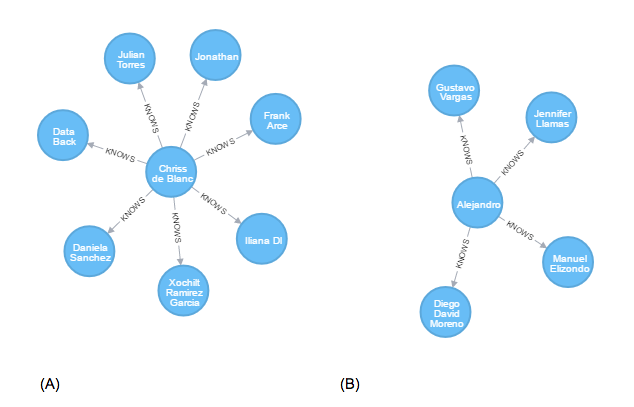
\includegraphics[scale=0.75]{img/users_known_1.PNG} %[width=0.7\textwidth]
\caption{Graph users with greater interconnectivity.}
\label{fig:guserknown_1}
\end{figure*}

Figure\ref{fig:guserknown_1} shows those users more connected in the graph. This
may represent the degree of impact of a user and the possible influence that may
have on the decisions of other users. For example, if the user with the greatest
impact is affected in any decision likely other users may be affected in some
way.


\begin{table}
\small
\caption{Total number of individuals generated.}
\label{tab:totalIndividuals_12}
\centering
\small
\begin{tabular}{p{3cm} p{3cm} p{3cm} }
\hline\noalign{\smallskip}
  & Individuals &  \\
\noalign{\smallskip}\hline\noalign{\smallskip}
\small{Total } & \small{500} & \\ \hline
\noalign{\smallskip}\hline
\end{tabular}
\end{table}


Table \ref{tab:totalIndividuals_12} presents the total number of individuals
generated within the graph.

\begin{table}
\small
\caption{Sample of 30 individuals evaluated from.}
\label{tab:totalIndividuals_1}
\centering
\small
\begin{tabular}{p{3cm} p{4cm} p{3cm} p{3cm}}
\hline\noalign{\smallskip}
 id & Chromosome & Views & Likes  \\
\noalign{\smallskip}\hline\noalign{\smallskip}
\small{pop:individual:107} & \small{[125, 30, 0, 1, 0, 0, 3, 0, 1, 0, 0, 0, 0, 2, 1]}
& \small{20} & \small{20}\\ \hline
\small{pop:individual:133} & \small{[143, 15, 1, 1, 0, 1, 3, 0, 1, 0, 2, 0, 0, 1, 1]}
& \small{15} & \small{15}\\ \hline
\small{pop:individual:109} & \small{[125, 30, 1, 1, 0, 0, 3, 0, 1, 0, 0, 0, 0, 0, 1]}
& \small{15} & \small{15}\\ \hline
\small{pop:individual:37} & \small{[87, 64, 1, 1, 1, 1, 4, 0, 1, 0, 0, 0, 1, 2, 3]}
& \small{14} & \small{14}\\ \hline
\small{pop:individual:36} & \small{[95, 71, 0, 1, 1, 0, 3, 1, 0, 0, 0, 1, 1, 1, 2]}
& \small{14} & \small{14}\\ \hline
\small{pop:individual:215} & \small{[138, 29, 1, 1, 0, 1, 3, 0, 1, 1, 1, 0, 0, 1, 1]}
& \small{13} & \small{13}\\ \hline
\small{pop:individual:228} & \small{[42, 58, 0, 0, 1, 1, 4, 0, 0, 0, 2, 0, 0, 0, 3]}
& \small{12} & \small{12}\\ \hline
\small{pop:individual:48} & \small{[51, 73, 0, 0, 0, 0, 2, 0, 0, 1, 3, 0, 1, 0, 3]}
& \small{12} & \small{12}\\ \hline
\small{pop:individual:39} & \small{[60, 12, 1, 1, 1, 1, 4, 1, 1, 1, 0, 1, 0, 1, 1]}
& \small{12} & \small{12}\\ \hline
\small{pop:individual:94} & \small{[49, 71, 0, 0, 1, 0, 4, 1, 0, 0, 1, 1, 1, 0, 2]}
& \small{11} & \small{11}\\ \hline
\small{pop:individual:194} & \small{[87, 64, 0, 1, 1, 1, 1, 3, 0, 0, 0, 0, 1, 2, 3]}
& \small{11} & \small{11}\\ \hline
\small{pop:individual:75} & \small{[97, 66, 0, 0, 1, 1, 3, 0, 1, 0, 3, 0, 1, 0, 1]}
& \small{11} & \small{11}\\ \hline
\small{pop:individual:105} & \small{[125, 30, 0, 1, 0, 0, 3, 0, 1, 0, 0, 1, 0, 0, 1]}
& \small{11} & \small{11}\\ \hline
\small{pop:individual:306} & \small{[87, 64, 1, 1, 1, 1, 4, 1, 1, 1, 1, 0, 1, 2, 3]}
& \small{13} & \small{10}\\ \hline
\small{pop:individual:326} & \small{[138, 29, 1, 1, 0, 1, 3, 0, 1, 1, 1, 0, 0, 0, 0]}
& \small{10} & \small{10}\\ \hline
\small{pop:individual:82} & \small{[81, 8, 1, 0, 0, 1, 4, 1, 1, 1, 2, 0, 0, 2, 1]}
& \small{10} & \small{10}\\ \hline
\small{pop:individual:252} & \small{[125, 30, 0, 1, 0, 0, 3, 0, 1, 1, 3, 0, 1, 0, 3]}
& \small{10} & \small{10}\\ \hline
\small{pop:individual:280} & \small{[53, 63, 1, 1, 0, 1, 3, 0, 1, 1, 0, 0, 0, 2, 1]}
& \small{9} & \small{9}\\ \hline
\small{pop:individual:178} & \small{[53, 63, 1, 1, 0, 1, 3, 0, 1, 1, 0, 0, 0, 2, 1]}
& \small{9} & \small{9}\\ \hline
\small{pop:individual:108} & \small{[42, 58, 0, 0, 1, 1, 3, 0, 1, 0, 1, 1, 0, 0, 1]}
& \small{10} & \small{9}\\ \hline
\small{pop:individual:231} & \small{[125, 30, 0, 1, 0, 0, 3, 0, 1, 1, 3, 0, 1, 0, 3]}
& \small{0} & \small{9}\\ \hline
\small{pop:individual:147} & \small{[122, 38, 1, 0, 0, 0, 0, 3, 0, 1, 0, 0, 0, 0, 0]}
& \small{9} & \small{9}\\ \hline
\small{pop:individual:181} & \small{[143, 15, 1, 1, 0, 1, 3, 0, 1, 0, 0, 0, 0, 0, 1]}
& \small{9} & \small{9}\\ \hline
\small{pop:individual:151} & \small{[49, 27, 1, 0, 0, 0, 3, 0, 0, 1, 2, 0, 1, 0, 3]}
& \small{9} & \small{9}\\ \hline
\small{pop:individual:34} & \small{[125, 30, 0, 1, 0, 0, 3, 0, 1, 0, 0, 0, 0, 2, 1]}
& \small{8} & \small{8}\\ \hline
\small{pop:individual:185} & \small{[122, 38, 0, 0, 0, 1, 1, 1, 1, 1, 3, 0, 1, 1, 1]}
& \small{8} & \small{8}\\ \hline
\small{pop:individual:88} & \small{[49, 62, 0, 1, 1, 1, 1, 1, 1, 1, 0, 0, 0, 2, 2]}
& \small{8} & \small{8}\\ \hline
\small{pop:individual:176} & \small{[125, 30, 0, 1, 0, 0, 3, 0, 1, 1, 3, 0, 1, 0, 3]}
& \small{8} & \small{8}\\ \hline
\small{pop:individual:234} & \small{[42, 58, 0, 0, 1, 1, 3, 0, 1, 0, 1, 0, 0, 0, 1]}
& \small{8} & \small{8}\\ \hline
\noalign{\smallskip}\hline
\end{tabular}
\end{table}

Table \ref{tab:totalIndividuals_1} contains a sample of 30/500 individuals were
generated in the experiment. Where we present the unique identifier of the
individual, its chromosome, as well as the number of views, likes available to
the individual. These results are useful to observe which individuals have been better
evaluated by users.

\begin{table}
\small
\caption{Level of user participation.}
\label{tab:userParticipation_1}
\centering
\small
\begin{tabular}{p{4cm} p{4cm}}
\hline\noalign{\smallskip}
 User name & Participation   \\
\noalign{\smallskip}\hline\noalign{\smallskip}
\small{Ana Laura Lopez} & \small{116} \\ \hline
\small{Mario García Valdez} & \small{100} \\ \hline
\small{Chriss de Blanc} & \small{93} \\ \hline
\small{Xochilt Ramirez Garcia} & \small{85} \\ \hline
\small{Carlos David Gallardo Pérez} & \small{73} \\ \hline
\small{Ulises Reus} & \small{70} \\ \hline
\small{Aaron Gutierrez Urbina} & \small{58} \\ \hline
\small{Cesar López} & \small{49} \\ \hline
\small{Hector Beltran Medrano} & \small{48} \\ \hline
\small{Luis Alfonso Felix Garcia} & \small{45} \\ \hline
\small{Data Back} & \small{39} \\ \hline
\small{Amaury Hernandez Aguila} & \small{32} \\ \hline
\small{Osmar Herrera Duran} & \small{31} \\ \hline
\small{Jorman Gtz} & \small{29} \\ \hline
\small{Alexis Campos Lopez} & \small{29} \\ \hline
\small{Melissa Muñoz Montes} & \small{28} \\ \hline
\small{David Gallegos} & \small{23} \\ \hline
\small{Jose Carlos} & \small{21} \\ \hline
\small{Tomás Perrín} & \small{21} \\ \hline
\small{Manuel Elizondo} & \small{20} \\ \hline


\noalign{\smallskip}\hline
\end{tabular}
\end{table}




Table \ref{tab:userParticipation_1} shows the results of the level of user
participation in the experiment. These were obtained by counting the vicinity of
nearest nodes from the base node in this case each user node.



\begin{figure*}
%\captionsetup{justification=centering,margin=1cm}
\centering
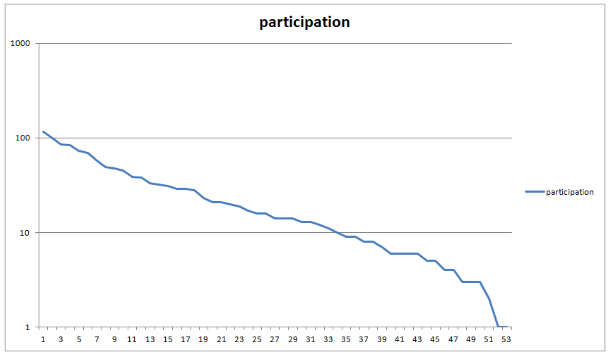
\includegraphics[scale=0.75]{img/Visual_represntation_1.PNG} %[width=0.7\textwidth]
\caption{Visual representation of user participation in EvoDrawing01.}
\label{fig:userP_1}
\end{figure*}

Figure \ref{fig:userP_1}  a visual representation of user
participation is presented, this experiment where the y-axis represents the level of
participation and the x-axis represents the number of users who participated in
this experiment.

\begin{figure*}
%\captionsetup{justification=centering,margin=1cm}
\centering
\fbox{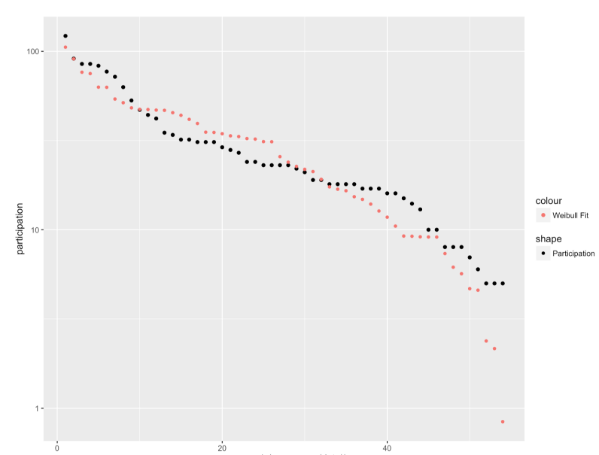
\includegraphics[scale=0.75]{img/weibull_1.PNG}} %[width=0.7\textwidth]
\caption{Weibull fit data representation.}
\label{fig:weibull_1}
\end{figure*}

For this particular experiment we were modeling with the Weibull distribution
\cite{weibull1951wide} the participation data of 53 users and these are the
results of the shape parameter and those of scale:

\begin{table}
\small
\caption{Weibull parameters.}
\label{tab:weibullp_1}
\centering
\small
\begin{tabular}{p{3cm} p{3cm} p{3cm} }
\hline\noalign{\smallskip}
Shape  & Scale &  \\
\noalign{\smallskip}\hline\noalign{\smallskip}
\small{0.9940324} & \small{25.4201542} & \\ \hline
\small{( 0.1036683)} & \small{( 3.7182494)} & \\ \hline

\noalign{\smallskip}\hline
\end{tabular}
\end{table}

Table \ref{tab:weibullp_1} shows the behavior in the Figure
\ref{fig:userP_1}, where the red dots are the adjustment of the Weibull
distribution and the black dots are the real data of the participations of the
users.



\section {EvoDrawing02}



Table \ref{tab:dataGenerated_2} shows the nodes and relatioships generated
by experiment ED02.

\begin{table}
\small
\caption{Data generated in graph-based user modeling.}
\label{tab:dataGenerated_2}
\centering
\small
\begin{tabular}{p{3cm} p{3cm} p{3cm} }
\hline\noalign{\smallskip}
  & Data &  \\
\noalign{\smallskip}\hline\noalign{\smallskip}
\small{Nodes} & \small{648} & \\ \hline
\small{Relationships} & \small{2596} & \\ \hline

\noalign{\smallskip}\hline
\end{tabular}
\end{table}
Also, the table\ref{tab:totalUsers_1} is the total of volunteer active users is
presented.

The total number of users who participate voluntarily is shown in the table \ref{tab:totalUsers_1}.

\begin{table}
\small
\caption{Total number of volunteers active users.}
\label{tab:totalUsers_1}
\centering
\small
\begin{tabular}{p{3cm} p{3cm} p{3cm} }
\hline\noalign{\smallskip}
  & Users &  \\
\noalign{\smallskip}\hline\noalign{\smallskip}
\small{Total } & \small{54} & \\ \hline
\noalign{\smallskip}\hline
\end{tabular}
\end{table}

Like in the previous experiment, in which we wanted to observe which users
had better social
interconnectivity within the experiment, it was decided to see this
relationship that corresponds to the number of known users. The table \ref{tab:totalUsers_1}
showed the relationships where the top 10 user  with social
interconnectivity for this particular experiment.


\begin{table}
\small
\caption{A sample of the top 10 users interconnected users.}
\label{tab:knownUsers_2}
\centering
\small
\begin{tabular}{p{3cm} p{3cm}  }
\hline\noalign{\smallskip}
 User name & Number of known users \\
\noalign{\smallskip}\hline\noalign{\smallskip}
\small{Rogelio UR} & \small{10}  \\ \hline
\small{Barbara Sandoval} & \small{9}  \\ \hline
\small{Evelyn Macedo} & \small{8}  \\ \hline
\small{Chriss de Blanc} & \small{8}  \\ \hline
\small{Cesar Rojas} & \small{8}  \\ \hline
\small{Jasiel Calzada} & \small{8}  \\ \hline
\small{Tonyy Maldonado} & \small{7}  \\ \hline
\small{Silvano Peraza} & \small{7}  \\ \hline
\small{Hector Beltran Medrano} & \small{6}  \\ \hline
\small{Juan Ferman Lopez} & \small{6}  \\ \hline
\noalign{\smallskip}\hline
\end{tabular}
\end{table}

Figure \ref{fig:userInter_2} shows users with more interconnectivity in the
graph. This may represent a certain degree of impact of a user and a possible influence
that may have on the decisions of other users. For example, if the
user with the greatest impact is affected in any decision likely other users may
be affected in some way. Particularly in this experiment the degree of social
interconnectivity among users is becoming more complex as compared to the
previous experiment.

\begin{figure*}
%\captionsetup{justification=centering,margin=1cm}
\centering
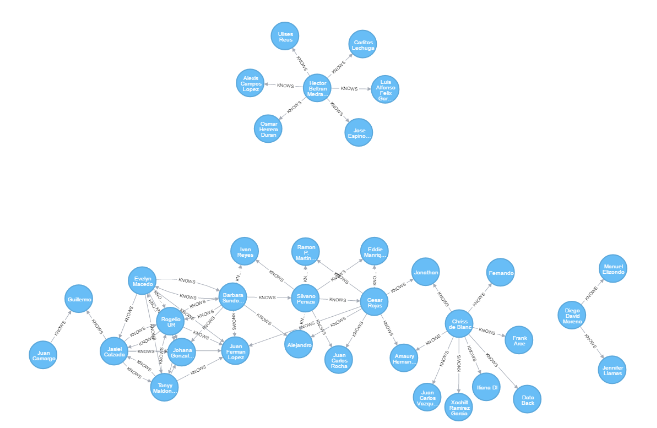
\includegraphics[scale=0.75]{img/user_known_2.PNG} %[width=0.7\textwidth]
\caption{Graph users with greater interconnectivity.}
\label{fig:userInter_2}
\end{figure*}

\begin{table}
\small
\caption{Sample of 30 individuals evaluated from.}
\label{tab:totalIndividuals_2}
\centering
\small
\begin{tabular}{p{3cm} p{4cm} p{3cm} p{3cm}}
\hline\noalign{\smallskip}
 id & Chromosome & Views & Likes  \\
\noalign{\smallskip}\hline\noalign{\smallskip}
\small{pop:individual:55} & \small{[63, 58, 0, 1, 1, 1, 4, 0, 0, 1, 0, 0, 0, 0, 3]}
& \small{18} & \small{18}\\ \hline
\small{pop:individual:329} & \small{[98, 37, 0, 1, 1, 0, 4, 0, 0, 1, 0, 0, 0, 0, 2]}
& \small{17} & \small{17}\\ \hline
\small{pop:individual:304} & \small{[63, 58, 0, 1, 1, 1, 4, 0, 0, 0, 3, 0, 0, 2, 2]}
& \small{16} & \small{16}\\ \hline
\small{pop:individual:202} & \small{[107, 79, 1, 0, 1, 1, 3, 0, 0, 1, 3, 0, 1, 1]}
& \small{15} & \small{15}\\ \hline
\small{pop:individual:58} & \small{[150, 79, 1, 0, 1, 1, 3, 0, 0, 1, 3, 0, 1, 1, 1]}
& \small{14} & \small{14}\\ \hline
\small{pop:individual:310} & \small{[63, 58, 0, 1, 1, 1, 4, 0, 0, 1, 0, 0, 1, 2, 2]}
& \small{13} & \small{13}\\ \hline
\small{pop:individual:67} & \small{[65, 51, 1, 1, 0, 0, 3, 1, 0, 0, 3, 1, 0, 2, 3]}
& \small{12} & \small{12}\\ \hline
\small{pop:individual:48} & \small{[51, 73, 0, 0, 0, 0, 2, 0, 0, 1, 3, 0, 1, 0, 3]}
& \small{12} & \small{12}\\ \hline
\small{pop:individual:179} & \small{[98, 37, 0, 1, 1, 1, 4, 0, 0, 1, 0, 0, 0, 0, 3]}
& \small{12} & \small{12}\\ \hline
\small{pop:individual:114} & \small{[63, 58, 0, 1, 1, 1, 4, 0, 0, 1, 0, 0, 0, 0, 2]}
& \small{12} & \small{12}\\ \hline
\small{pop:individual:123} & \small{[124, 42, 0, 1, 1, 1, 4, 1, 0, 1, 1, 0, 0, 2, 1]}
& \small{12} & \small{12}\\ \hline
\small{pop:individual:344} & \small{[97, 66, 0, 0, 1, 1, 3, 0, 1, 0, 3, 0, 1, 0, 1]}
& \small{11} & \small{11}\\ \hline
\small{pop:individual:105} & \small{[63, 58, 0, 1, 1, 1, 4, 0, 0, 1, 0, 0, 0, 0, 2]}
& \small{11} & \small{11}\\ \hline
\small{pop:individual:435} & \small{[98, 37, 0, 1, 1, 0, 1, 1, 4, 1, 0, 0, 0, 0, 2]}
& \small{11} & \small{11}\\ \hline
\small{pop:individual:140} & \small{[150, 79, 1, 0, 1, 1, 3, 1, 1, 0, 1, 1, 1, 2, 3]}
& \small{11} & \small{11}\\ \hline
\small{pop:individual:216} & \small{[124, 42, 0, 1, 0, 0, 3, 0, 0, 1, 1, 0, 0, 1, 1]}
& \small{11} & \small{11}\\ \hline
\small{pop:individual:290} & \small{[150, 79, 1, 0, 1, 1, 3, 0, 0, 1, 3, 0, 1, 0, 1]}
& \small{10} & \small{10}\\ \hline
\small{pop:individual:255} & \small{[150, 79, 1, 0, 1, 1, 3, 1, 1, 1, 0, 0, 1, 2, 2]}
& \small{10} & \small{10}\\ \hline
\small{pop:individual:14} & \small{[89, 66, 0, 0, 1, 1, 3, 0, 0, 0, 2, 0, 0, 2, 1]}
& \small{10} & \small{10}\\ \hline
\small{pop:individual:366} & \small{[128, 66, 0, 1, 1, 4, 1, 0, 1, 0, 0, 0, 1, 2, 2]}
& \small{10} & \small{10}\\ \hline
\small{pop:individual:215} & \small{[54, 72, 0, 1, 1, 1, 4, 0, 0, 1, 0, 0, 0, 0, 2]}
& \small{9} & \small{9}\\ \hline
\small{pop:individual:411} & \small{[113, 58, 0, 1, 1, 1, 4, 0, 0, 1, 0, 0, 1, 2, 2]}
& \small{9} & \small{9}\\ \hline
\small{pop:individual:254} & \small{[113, 58, 0, 1, 1, 4, 1, 0, 4, 1, 1, 0, 0, 3]}
& \small{11} & \small{9}\\ \hline
\small{pop:individual:285} & \small{[54, 58, 0, 0, 0, 1, 1, 4, 1, 1, 0, 0, 1, 2, 2]}
& \small{8} & \small{8}\\ \hline
\small{pop:individual:500} & \small{[63, 58, 1, 1, 1, 0, 3, 0, 1, 1, 0, 0, 1, 2, 0]}
& \small{8} & \small{8}\\ \hline
\small{pop:individual:415} & \small{[54, 72, 0, 1, 1, 1, 4, 1, 4, 1, 3, 0, 1, 1]}
& \small{8} & \small{8}\\ \hline
\small{pop:individual:300} & \small{[54, 58, 1, 0, 1, 1, 1, 4, 1, 1, 0, 0, 1, 2, 2]}
& \small{8} & \small{8}\\ \hline
\small{pop:individual:32} & \small{[113, 29, 0, 0, 0, 0, 4, 1, 0, 1, 0, 1, 1, 1, 3]}
& \small{8} & \small{8}\\ \hline
\small{pop:individual:237} & \small{[63, 58, 1, 1, 0, 1, 1, 4, 1, 0, 0, 0, 1, 2, 3]}
& \small{8} & \small{8}\\ \hline
\small{pop:individual:268} & \small{[98, 37, 0, 1, 1, 1, 4, 0, 0, 1, 0, 0, 0, 0]}
& \small{8} & \small{8}\\ \hline
\noalign{\smallskip}\hline
\end{tabular}
\end{table}

Table \ref{tab:totalIndividuals_2} contains a sample of individuals 30/556
generated in the experiment. This table shows the unique identifier of the
individual, its chromosome, as well as the number of views, likes available to
the individual. These results are useful to observe individuals have been better
evaluated by users.

\begin{table}
\small
\caption{Level of user participation.}
\label{tab:userParticipation_2}
\centering
\small
\begin{tabular}{p{4cm} p{4cm}}
\hline\noalign{\smallskip}
 User name & Participation   \\
\noalign{\smallskip}\hline\noalign{\smallskip}
\small{1122212314475816} & \small{122} \\ \hline
\small{1107674982600275} & \small{91} \\ \hline
\small{10207544086753085} & \small{86} \\ \hline
\small{1128990193799346} & \small{85} \\ \hline
\small{1067084180030552} & \small{83} \\ \hline
\small{985591718197586} & \small{77} \\ \hline
\small{969507913124553} & \small{72} \\ \hline
\small{10207004677610003} & \small{63} \\ \hline
\small{1223229694371825} & \small{53} \\ \hline
\small{10153904046011462} & \small{47} \\ \hline
\small{1032494570125948} & \small{44} \\ \hline
\small{995610090523549} & \small{42} \\ \hline
\small{975038365907627} & \small{35} \\ \hline
\small{10207487295119454} & \small{34} \\ \hline
\small{1041989022528624} & \small{32} \\ \hline
\small{471974623003503} & \small{32} \\ \hline
\small{1275844349097672} & \small{31} \\ \hline
\small{978744228875903} & \small{31} \\ \hline
\small{10205734318020434} & \small{31} \\ \hline
\small{10209454397419860} & \small{29} \\ \hline


\noalign{\smallskip}\hline
\end{tabular}
\end{table}

Table \ref{tab:userParticipation_2} shows the results of the level of user
participation in the experiment. These were obtained by counting the vicinity of
nearest nodes from the base node, in this case, each user node.


\begin{figure*}
%\captionsetup{justification=centering,margin=1cm}
\centering
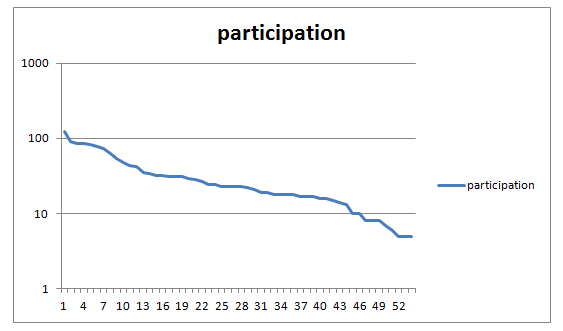
\includegraphics[scale=0.75]{img/visual_representation_2.PNG} %[width=0.7\textwidth]
\caption{Visual representation of user participation in EvoDrawing01.}
\label{fig:userP_2}
\end{figure*}


Figure \ref{fig:userP_2} shows a visual representation of user
participation in this experiment where the y-axis represents the level of
participation and the x-axis represents the number of users who participated in
this experiment.

\begin{figure*}
%\captionsetup{justification=centering,margin=1cm}
\centering
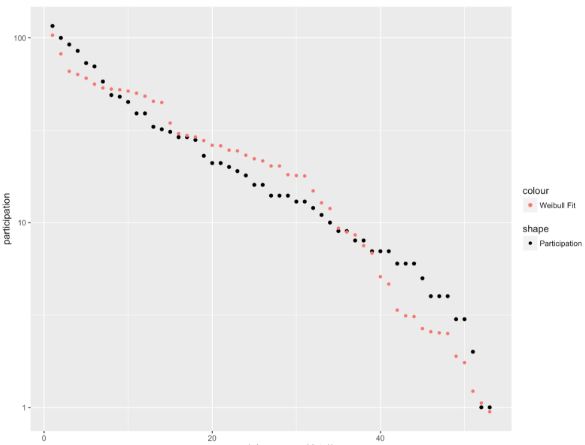
\includegraphics[scale=0.75]{img/weibull_2.PNG} %[width=0.7\textwidth]
\caption{Weibull fit data representation.}
\label{fig:weibull_2}
\end{figure*}

For this particular experiment we were modeling with the Weibull distribution
\cite{weibull1951wide} the participation data of 54 users and these are the
results of the shape and the scale parameter:

\begin{table}
\small
\caption{Weibull parameters.}
\label{tab:weibullp_2}
\centering
\small
\begin{tabular}{p{3cm} p{3cm} p{3cm} }
\hline\noalign{\smallskip}
Shape  & Scale &  \\
\noalign{\smallskip}\hline\noalign{\smallskip}
\small{1.3255300} & \small{33.7680210} & \\ \hline
\small{(0.1330041)} & \small{(3.6776628)} & \\ \hline

\noalign{\smallskip}\hline
\end{tabular}
\end{table}

Table \ref{tab:weibullp_2} shows the behavior, Figure
\ref{fig:weibull_2} show Weibull distribution, where the red dots are the adjustment of the Weibull
distribution and the black dots are the real data of the participations of the
users.




\section{EvoDrawing03}
In the experiment ED03 the following data were
generated presented in \ref{tab:dataGenerated_3}.

\begin{table}
\small
\caption{Data generated in graph-based user modeling.}
\label{tab:dataGenerated_3}
\centering
\small
\begin{tabular}{p{3cm} p{3cm} p{3cm} }
\hline\noalign{\smallskip}
  & Data &  \\
\noalign{\smallskip}\hline\noalign{\smallskip}
\small{Nodes} & \small{3746 } & \\ \hline
\small{Relationships} & \small{17207 } & \\ \hline

\noalign{\smallskip}\hline
\end{tabular}
\end{table}

The total number of users who participate voluntarily shown in \ref{tab:totalUsers_3}.

\begin{table}
\small
\caption{Total number of volunteers active users.}
\label{tab:totalUsers_3}
\centering
\small
\begin{tabular}{p{3cm} p{3cm} p{3cm} }
\hline\noalign{\smallskip}
  & Users &  \\
\noalign{\smallskip}\hline\noalign{\smallskip}
\small{Total } & \small{68} & \\ \hline
\noalign{\smallskip}\hline
\end{tabular}
\end{table}

In the same way as the previous experiment, which wanted to observe users, had
better social interconnectivity within this experiment, it was decided a known
ratio of the number of users that have. This relationship is presented in Table
\ref{tab:knownUsers_3}  where we show the 10 users with better social
interconnectivity.

\begin{table}
\small
\caption{A sample of the top 10 users level influence on users.}
\label{tab:knownUsers_3}
\centering
\small
\begin{tabular}{p{3cm} p{3cm}  }
\hline\noalign{\smallskip}
 User name & Number of known users \\
\noalign{\smallskip}\hline\noalign{\smallskip}
\small{David Astorga Viramontes} & \small{23}  \\ \hline
\small{Evelyn Macedo} & \small{18}  \\ \hline
\small{Reyes Zuniga} & \small{17}  \\ \hline
\small{Barbara Sandoval} & \small{16}  \\ \hline
\small{Chriss de Blanc} & \small{15}  \\ \hline
\small{Luis Alfonso Felix Garcia} & \small{15}  \\ \hline
\small{Paulina NG} & \small{15}  \\ \hline
\small{Marco Antonio Fuentes Alvarez} & \small{15}  \\ \hline
\small{Jasiel Calzada} & \small{14}  \\ \hline
\small{Hector Beltran Medrano} & \small{13}  \\ \hline
\noalign{\smallskip}\hline
\end{tabular}
\end{table}


\begin{figure*}
%\captionsetup{justification=centering,margin=1cm}
\centering
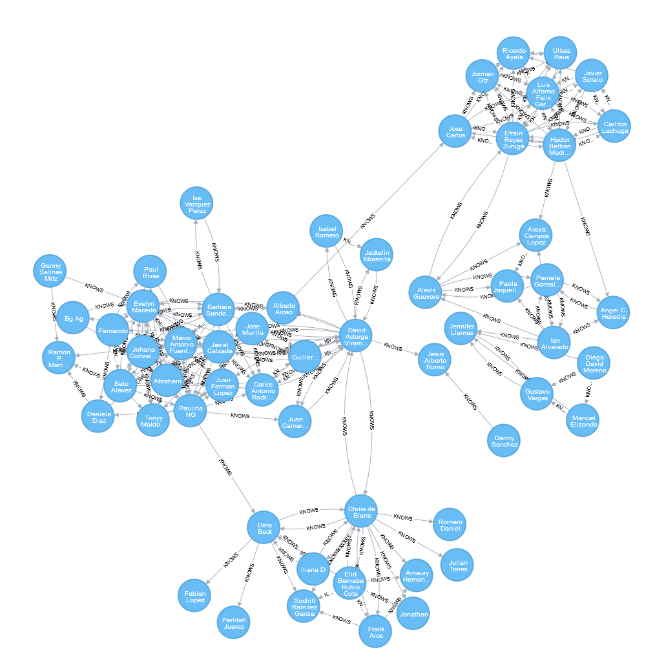
\includegraphics[scale=0.75]{img/user_known_3.PNG} %[width=0.7\textwidth]
\caption{Social interconnectivity in graph-based user model.}
\label{fig:graphKnown_3}
\end{figure*}

Figure \ref{fig:graphKnown_3} shows users more connected in the graph. This
may represent a degree of impact of a user and the possible influence that may
have on the decisions of other users. For example, if the user with the greatest
impact is affected in any decision likely other users may be affected in some
way. Particularly in this experiment the social graph interconnectivity among
users is becoming more complex as compared to the previous experiment as we can
observe that more closely resembles a social network.


\begin{table}
\small
\caption{Total number of individuals.}
\label{tab:totalIndividuals_33}
\centering
\small
\begin{tabular}{p{3cm} p{3cm} p{3cm} }
\hline\noalign{\smallskip}
  & Individuals &  \\
\noalign{\smallskip}\hline\noalign{\smallskip}
\small{Total } & \small{3594} & \\ \hline
\noalign{\smallskip}\hline
\end{tabular}
\end{table}

Table \ref{tab:totalIndividuals_33} shows the total number of individuals
evaluated by users in this experiment.

\begin{table}
\small
\caption{Sample of 30 individuals evaluated from.}
\label{tab:totalIndividuals_32}
\centering
\small
\begin{tabular}{p{3cm} p{4cm} p{3cm} p{3cm}}
\hline\noalign{\smallskip}
 id & Chromosome & Views & Likes  \\
\noalign{\smallskip}\hline\noalign{\smallskip}
\small{pop:individual:3570} & \small{[113, 44, 0, 1, 0, 0, 1, 0, 1, 0, 3, 1, 1, 0, 1]}
& \small{48} & \small{48}\\ \hline
\small{pop:individual:3544} & \small{[150, 44, 0, 0, 1, 1, 1, 0, 0, 1, 1, 0, 1, 0, 0]}
& \small{32} & \small{26}\\ \hline
\small{pop:individual:210} & \small{[63, 58, 0, 1, 1, 1, 4, 0, 0, 0, 3, 0, 0, 2, 2]}
& \small{16} & \small{16}\\ \hline
\small{pop:individual:202} & \small{[113, 5, 0, 1, 1, 0, 4, 0, 1, 1, 2, 1, 0, 2, 2]}
& \small{22} & \small{22}\\ \hline
\small{pop:individual:58} & \small{[61, 70, 0, 0, 1, 0, 1, 0, 0, 0, 2, 0, 1, 0, 3]}
& \small{23} & \small{21}\\ \hline
\small{pop:individual:858} & \small{[113, 1, 1, 1, 1, 0, 1, 1, 1, 3, 0, 1, 1, 0]}
& \small{21} & \small{21}\\ \hline
\small{pop:individual:17} & \small{[113, 69, 0, 1, 1, 1, 3, 0, 1, 1, 0, 0, 1, 0, 3]}
& \small{23} & \small{21}\\ \hline
\small{pop:individual:3636} & \small{[118, 44, 0, 0, 1, 1, 1, 0, 0, 1, 1, 1, 1, 0, 0]}
& \small{22} & \small{21}\\ \hline
\small{pop:individual:33} & \small{[129, 79, 0, 1, 1, 0, 1, 1, 0, 0, 0, 1, 0, 0, 1]}
& \small{20} & \small{20}\\ \hline
\small{pop:individual:74} & \small{[150, 50, 1, 1, 1, 1, 1, 1, 0, 1, 3, 1, 0, 1, 3]}
& \small{21} & \small{19}\\ \hline
\small{pop:individual:65} & \small{[94, 62, 1, 0, 0, 0, 2, 0, 1, 0, 3, 0, 1, 2, 2]}
& \small{20} & \small{19}\\ \hline
\small{pop:individual:50} & \small{[50, 70, 0, 1, 1, 1, 3, 1, 1, 1, 1, 1, 1, 1, 3]}
& \small{19} & \small{19}\\ \hline
\small{pop:individual:52} & \small{[131, 63, 1, 1, 1, 0, 4, 0, 1, 1, 0, 0, 1, 0, 3]}
& \small{20} & \small{19}\\ \hline
\small{pop:individual:2449} & \small{[113, 44, 0, 1, 1, 1, 1, 0, 1, 1, 0, 0, 1, 1, 2]}
& \small{18} & \small{18}\\ \hline
\small{pop:individual:44} & \small{[117, 54, 0, 0, 0, 0, 2, 0, 1, 1, 3, 1, 0, 2, 3]}
& \small{19} & \small{18}\\ \hline
\small{pop:individual:113} & \small{[77, 21, 1, 0, 1, 0, 4, 0, 1, 0, 0, 1, 0, 3]}
& \small{17} & \small{17}\\ \hline
\small{pop:individual:84} & \small{[102, 69, 1, 0, 1, 0, 3, 0, 0, 0, 0, 0, 1, 0, 3]}
& \small{17} & \small{17}\\ \hline
\small{pop:individual:95} & \small{[68, 43, 0, 1, 0, 1, 3, 1, 0, 0, 3, 0, 0, 1, 2]}
& \small{19} & \small{16}\\ \hline
\small{pop:individual:22} & \small{[137, 20, 0, 0, 0, 0, 0, 1, 0, 0, 3, 0, 1, 1, 1]}
& \small{17} & \small{16}\\ \hline
\small{pop:individual:71} & \small{[79, 5, 0, 0, 1, 1, 2, 1, 0, 1, 0, 1, 1, 1, 3]}
& \small{16} & \small{16}\\ \hline
\small{pop:individual:42} & \small{[112, 35, 1, 0, 1, 0, 1, 0, 1, 0, 0, 1, 1, 0, 2]}
& \small{9} & \small{9}\\ \hline
\small{pop:individual:411} & \small{[113, 58, 0, 1, 1, 1, 4, 0, 0, 1, 0, 0, 1, 2, 2]}
& \small{16} & \small{15}\\ \hline
\small{pop:individual:59} & \small{[93, 23, 0, 0, 0, 1, 4, 0, 0, 0, 1, 0, 1, 2, 1]}
& \small{17} & \small{15}\\ \hline
\small{pop:individual:40} & \small{[137, 9, 1, 0, 1, 0, 3, 0, 1, 1, 2, 0, 1, 2, 1]}
& \small{15} & \small{15}\\ \hline
\small{pop:individual:85} & \small{[120, 42, 0, 1, 0, 1, 0, 0, 1, 1, 3, 0, 1, 1, 2]}
& \small{16} & \small{15}\\ \hline
\small{pop:individual:90} & \small{[130, 76, 0, 0, 1, 1, 1, 1, 1, 1, 1, 0, 1, 2, 3]}
& \small{15} & \small{15}\\ \hline
\small{pop:individual:73} & \small{[88, 67, 0, 0, 0, 0, 0, 1, 1, 1, 2, 1, 0, 1, 3]}
& \small{15} & \small{15}\\ \hline
\small{pop:individual:943} & \small{[116, 44, 0, 0, 0, 4, 1, 1, 1, 1, 0, 1, 0, 1, 1]}
& \small{15} & \small{15}\\ \hline
\small{pop:individual:353} & \small{[121, 20, 1, 1, 0, 0, 1, 0, 1, 1, 3, 0, 1, 0, 2]}
& \small{15} & \small{15}\\ \hline
\small{pop:individual:79} & \small{[68, 5, 1, 1, 0, 1, 1, 1, 1, 0, 2, 1, 1, 1, 1]}
& \small{14} & \small{14}\\ \hline
\noalign{\smallskip}\hline
\end{tabular}
\end{table}

Table \ref{tab:totalIndividuals_32} contains a sample of individuals 30/556
generated in the experiment. In this, its a unique identifier of the individual,
its chromosome, as well as the number of views, likes available to the individual presents.
This results, which are useful to observe individuals have been better evaluated by users.

\begin{table}
\small
\caption{Level of user participation.}
\label{tab:userParticipation_22}
\centering
\small
\begin{tabular}{p{4cm} p{4cm}}
\hline\noalign{\smallskip}
 User name & Participation   \\
\noalign{\smallskip}\hline\noalign{\smallskip}
\small{1157401414272355} & \small{2035} \\ \hline
\small{1001585659925992} & \small{1828} \\ \hline
\small{1244770712203948} & \small{1722} \\ \hline
\small{990632971026794} & \small{552} \\ \hline
\small{987920194610578} & \small{456} \\ \hline
\small{10207675081608741} & \small{300} \\ \hline
\small{966757780068615} & \small{267} \\ \hline
\small{1228561717171956} & \small{258} \\ \hline
\small{985416538190778} & \small{203} \\ \hline
\small{1123938694291507} & \small{202} \\ \hline
\small{10207552420841432} & \small{200} \\ \hline
\small{1124138344283213} & \small{169} \\ \hline
\small{220415891643957} & \small{161} \\ \hline
\small{534039336778842} & \small{112} \\ \hline
\small{10153940958696462} & \small{93} \\ \hline
\small{10205543461172072} & \small{87} \\ \hline
\small{1281817738500333} & \small{81} \\ \hline
\small{10153866481615259} & \small{74} \\ \hline
\small{943775989063530} & \small{73} \\ \hline
\small{10205664691039169} & \small{71} \\ \hline


\noalign{\smallskip}\hline
\end{tabular}
\end{table}

Figure \ref{fig:userP_3} shows a visual representation of user participation
of this experiment where the y-axis represents the level of participation and
the x-axis represents the number of users who participated in this experiment.

\begin{figure*}
%\captionsetup{justification=centering,margin=1cm}
\centering
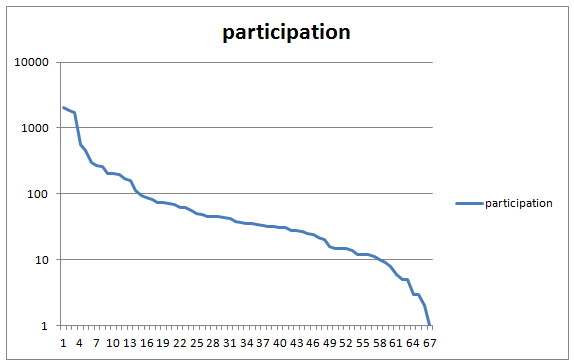
\includegraphics[scale=0.75]{img/visual_representation_3.PNG} %[width=0.7\textwidth]
\caption{Visual representation of user participation in EvoDrawing01.}
\label{fig:userP_3}
\end{figure*}


\begin{figure*}
%\captionsetup{justification=centering,margin=1cm}
\centering
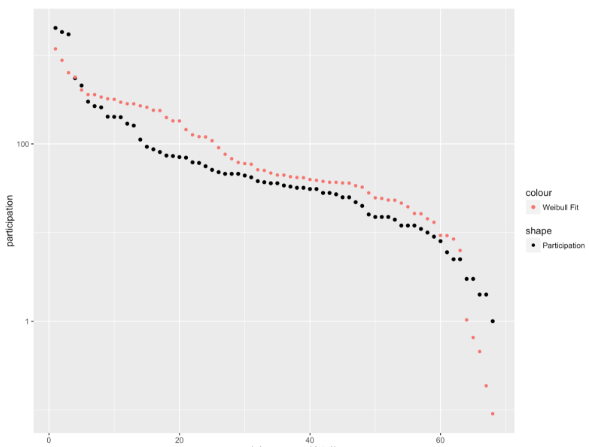
\includegraphics[scale=0.75]{img/weibull_3.PNG} %[width=0.7\textwidth]
\caption{Weibull fit data representation.}
\label{fig:weibull_3}
\end{figure*}

For this particular experiment we were modeling with the Weibull distribution
\cite{weibull1951wide} the participation data of 68 users and these are the
results of the shape and scale parameter:

\begin{table}
\small
\caption{Weibull parameters.}
\label{tab:weibullp_3}
\centering
\small
\begin{tabular}{p{3cm} p{3cm} p{3cm} }
\hline\noalign{\smallskip}
Shape  & Scale &  \\
\noalign{\smallskip}\hline\noalign{\smallskip}
\small{0.6027560} & \small{85.0232792} & \\ \hline
\small{(0.0507141)} & \small{(18.1151136)} & \\ \hline

\noalign{\smallskip}\hline
\end{tabular}
\end{table}

Table \ref{tab:weibullp_3} shows the behavior in the Figure
\ref{fig:weibull_3}, where the red dots are the adjustment of the Weibull
distribution and the black dots are the real data of the participations of the
users.



\section{Comparison between experiments}
% Figure \ref{fig:comparison} shows a comparative chart of the results obtained
% in the three phases of the study case, each of the lines on the graph represents
% one of the versions of EvoDrawing in relation to the number of units of users
% that were obtained are presented in different experiments. For instance the blue
% line represents ED1 experiment, the red line represents ED02
% and finally the green line represents ED03.

Figure \ref{fig:comparison} shows a chart of the results obtained in the three
phases of the study case, where each line represents the participation of the
users of their respective version of Evo-Drawings. This chart is on a
logarithmic scale in the y-axis and represents the participation of the users,
as well as the x-axis, that represents the number of users that participated.
For instance, the blue line represents the experiment ED01 which had a max value
of 116 participations And a minimum of 1 participation, also had a maximum of 54
participants and a minimum of 1. In this sense the red line represents the
experiment ED02 which obtained a max value of 122 participations and a minimum
of 8, also had a max value of 56 participants and a minimum of 1 participant.
Finally, the green line represents the experiment ED03 which obtained a max
value of 2035 participations and a minimum of 1 participation, also had a max
value of 67 participants and a minimum of one participant.

\begin{figure*}
%\captionsetup{justification=centering,margin=1cm}
\centering
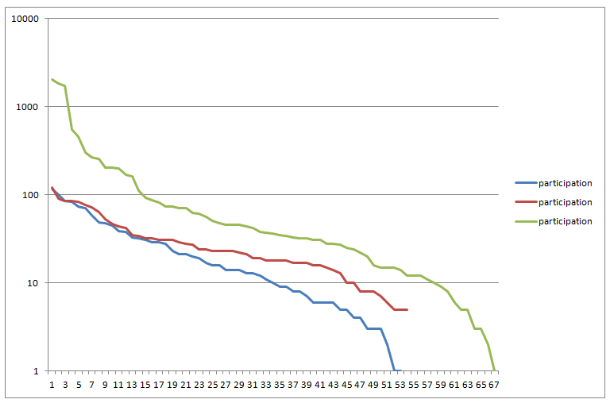
\includegraphics[scale=0.75]{img/comparison.PNG} %[width=0.7\textwidth]
\caption{Graphical representation of user participation in the different experiments.}
\label{fig:comparison}
\end{figure*}

\chapter{Conclusions and future work} \label{sec:5}

\section{Conclusions}

Using a user model in Web-based interactive evolutionary computation  overall with the different approaches such as fuzzy logic and gamification it demonstrated  in experiment EvoDrawing03 that the users increase their participation with respect to other versions (EvoDrawing01, EvoDrawin02).

In this sense the results have shown a phenomenon in the users which is competitiveness. This phenomenon occurs naturally because as human beings is our nature to be competitive regardless of the topic or activity that we assign [Reference]. This gave support to users return to evaluate more individuals within the experiment EvoDrawings03 and consequently the participation increase exponentially. 

In this research work also found that the way individuals was presented to be evaluated and how to evaluate them helped the user to take their evaluations so easy and quick. This means that users evaluated on average 40 or more individuals in an iteration, reducing the risk of demotivation assessment and therefore lose interest in participation. However, it was concluded that the biggest problem of interactive evolutionary computing systems remains on user fatigue.

The fatigue can be generated by many factors, such as how to evaluate individuals, the subject of the application, how to present the individuals, the objective within the application, expertise by users, and more. The resulting method of this research helps motivate users on the issue of participation in interactive evolutionary computing applications.


\section{Future work}



\prefacesection{Publications}
%\begin{singlespace}
\begin{enumerate}
\item \textit{User Modeling for Interactive Evolutionary Computation
Applications Using Fuzzy Logic. JC Romero, Mario Garc\'ia-Vald\'ez.
 Recent Advances on Hybrid Intelligent Systems. Springer Berlin Heidelberg. (2013)}
\item \textit{ EvoSpace-i: a framework for interactive evolutionary algorithms.
Mario Garc\'ia-Vald\'ez, 	Juan J. Merelo, 	Leonardo Trujillo, 	Francisco
Fernández-de-Vega Jos\'e C. Romero, 	Alejandra Mancilla. GECCO '13 Companion
Proceedings of the 15th annual conference  companion on Genetic and evolutionary
computation. Amsterdam, The Netherlands. (2013).}
\item \textit{Using a Graph Based Database to Support Collaborative Interactive
Evolutionary Systems.  JC Romero, Mario Garc\'ia-Vald\'ez. Recent Advances on
Hybrid Approaches for Designing Intelligent Systems. Springer International
Publishing Switzerland. Volume 547 of the series Studies in Computational
Intelligence pp 581-591. Switzerland. (2014).}
\item \textit{A Fitness Estimation Strategy for Web Based Interactive Evolutionary
Applications Considering User Preferences and Activities Using Fuzzy Logic. J.C.
Romero, Mario Garc\'ia-Vald\'ez. Design of Intelligent Systems Based on Fuzzy
Logic, Neural Networks and Nature-Inspired Optimization. Springer International
Publishing Switzerland. Volume 601 of the series Studies in Computational
Intelligence pp 507-516. (2015).}
\item \textit{Modeling Human Interactions in
Collaborative Interactive Evolutionary Computation.  Mario Garc\'ia-Vald\'ez,
Christian Romero, Juan. J. Merelo, Alejandra Mancilla.  In Proceedings of the Genetic and Evolutionary Computation
Conference 2017, Berlin, Germany, July 15-19, 2017 (GECCO ’17).}
\item \textit{Exploiting the Social Graph: Increasing Engagement in a Collaborative Interactive Evolution Applications.
Mario Garc\'ia-Vald\'ez,
Christian Romero, Juan. J. Merelo, Alejandra Mancilla.  In Proceedings of IEEE Congress on Evolutionary Computation 2017
Donostia - San Sebastián, Spain
June 5-8, 2017.}
\end{enumerate}
%\end{singlespace}

\appendix
\chapter{EvoDrawing deploy instructions}\label{apendixa}

This section the instructions for deploying the EvoDrawings application are described.

\begin{enumerate}


\item \textit{First you need to clone the evodrawings
applications from github repository like this: In command promp put this:
git clone \url{https://github.com/jcromerohdz/evoDrawing_gaming.git/}. }


\item \textit{
Generate a repository on github service, if you don’t know how to create a
repository on github, here is a reference to help you create one \cite{}}

\item\textit{Generate an account on Heroku site.}

\item \textit{Go to applications and create one, this application can contain
any name you want in our particular case is evodrawings, after that you proceed
to link the heroku application with github service. Heroku service it’s gonna
ask you to provide permissions in order to connect to the github repository.}

\item \textit{Then find the manual deploy option on the application settings on
heroku, in figure x shows this section on the heroku application settings.}

\item \textit{Now you have to enable two add-ons services on heroku.
First one is the graphene service, you can choose the free one
The secound is the redis to go service, also you can choose the free one.}

\item \textit{To do the previous you have to do the following, first go to your heroku
settings and find the add-on option, the finds the service you want and select
the plan for both services.}





\end{enumerate}


\chapter{Fuzzy IF-THEN rules.}\label{apendixb}

This section presents the if-the rules used in the ED03 application.

\begin{enumerate}
	\item \textit{If \textbf{preference} is low and
		\textbf{experience} is low and \textbf{ranking} is low then \textbf{fuzzy-rate} is bad.}
	\item \textit{If \textbf{preference} is low and
		\textbf{experience} is low and \textbf{ranking} is mid then \textbf{fuzzy-rate} is bad.}
	\item \textit{If \textbf{preference} is low and
		\textbf{experience} is low and \textbf{ranking} is high then \textbf{fuzzy-rate} is bad.}
	\item \textit{If \textbf{preference} is low and
		\textbf{experience} is mid and \textbf{ranking} is low then \textbf{fuzzy-rate} is bad.}
	\item \textit{If \textbf{preference} is low and
		\textbf{experience} is mid and \textbf{ranking} is mid then \textbf{fuzzy-rate} is bad.}
	\item \textit{If \textbf{preference} is low and
		\textbf{experience} is mid and \textbf{ranking} is high then \textbf{fuzzy-rate} is normal.}
	\item \textit{If \textbf{preference} is low and
		\textbf{experience} is high and \textbf{ranking} is low then \textbf{fuzzy-rate} is normal.}
	\item \textit{If \textbf{preference} is low and
		\textbf{experience} is high and \textbf{ranking} is mid then \textbf{fuzzy-rate} is normal.}
	\item \textit{If \textbf{preference} is low and
		\textbf{experience} is high and \textbf{ranking} is high then \textbf{fuzzy-rate} is normal.}
	\item \textit{If \textbf{preference} is mid and
		\textbf{experience} is low and \textbf{ranking} is low then \textbf{fuzzy-rate} is bad.}
	\item \textit{If \textbf{preference} is mid and
		\textbf{experience} is low and \textbf{ranking} is mid then \textbf{fuzzy-rate} is normal.}
	\item \textit{If \textbf{preference} is mid and
		\textbf{experience} is low and \textbf{ranking} is high then \textbf{fuzzy-rate} is normal.}
	\item \textit{If \textbf{preference} is mid and
		\textbf{experience} is mid and \textbf{ranking} is low then \textbf{fuzzy-rate} is normal.}
	\item \textit{If \textbf{preference} is mid and
		\textbf{experience} is mid and \textbf{ranking} is mid then \textbf{fuzzy-rate} is normal.}
	\item \textit{If \textbf{preference} is mid and
		\textbf{experience} is mid and \textbf{ranking} is high then \textbf{fuzzy-rate} is normal.}
	\item \textit{If \textbf{preference} is mid and
		\textbf{experience} is high and \textbf{ranking} is low then \textbf{fuzzy-rate} is normal.}
	\item \textit{If \textbf{preference} is mid and
		\textbf{experience} is high and \textbf{ranking} is mid then \textbf{fuzzy-rate} is normal.}
	\item \textit{If \textbf{preference} is mid and
		\textbf{experience} is high and \textbf{ranking} is high then \textbf{fuzzy-rate} is normal.}
	\item \textit{If \textbf{preference} is high and
		\textbf{experience} is low and \textbf{ranking} is low then \textbf{fuzzy-rate} is normal.}\
	\item \textit{If \textbf{preference} is high and
		\textbf{experience} is low and \textbf{ranking} is mid then \textbf{fuzzy-rate} is normal.}\
	\item \textit{If \textbf{preference} is high and
		\textbf{experience} is low and \textbf{ranking} is high then \textbf{fuzzy-rate} is good.}\
	\item \textit{If \textbf{preference} is high and
		\textbf{experience} is mid and \textbf{ranking} is low then \textbf{fuzzy-rate} is normal.}\
	\item \textit{If \textbf{preference} is high and
		\textbf{experience} is mid and \textbf{ranking} is mid then \textbf{fuzzy-rate} is normal.}\
	\item \textit{If \textbf{preference} is high and
		\textbf{experience} is mid and \textbf{ranking} is high then \textbf{fuzzy-rate} is good.}\
	\item \textit{If \textbf{preference} is high and
		\textbf{experience} is high and \textbf{ranking} is low then \textbf{fuzzy-rate} is good.}\
	\item \textit{If \textbf{preference} is high and
		\textbf{experience} is high and \textbf{ranking} is mid then \textbf{fuzzy-rate} is good.}\
	\item \textit{If \textbf{preference} is high and
		\textbf{experience} is high and \textbf{ranking} is high then \textbf{fuzzy-rate} is good.}\

\end{enumerate}





%% Cap'itulos incluidos despues del comando \appendix aparecen como ap'endices
%% de la tesis.
%\include{apendiceB}
%\include{apendiceC}

%% Incluir la bibliograf'ia. Mirar el archivo "biblio.bib" para m'as detales
%% y un ejemplo.
\bibliography{biblio}

\end{document}
%%% SECCION DE APENDICE 
\prefacesection{Appendix}
